\documentclass[
11pt, % The default document font size, options: 10pt, 11pt, 12pt
oneside, % Two side (alternating margins) for binding by default, uncomment to switch to one side
english, % ngerman for German
singlespacing, % Single line spacing, alternatives: onehalfspacing or doublespacing
%draft, % Uncomment to enable draft mode (no pictures, no links, overfull hboxes indicated)
%nolistspacing, % If the document is onehalfspacing or doublespacing, uncomment this to set spacing in lists to single
%liststotoc, % Uncomment to add the list of figures/tables/etc to the table of contents
%toctotoc, % Uncomment to add the main table of contents to the table of contents
%parskip, % Uncomment to add space between paragraphs
%nohyperref, % Uncomment to not load the hyperref package
headsepline, % Uncomment to get a line under the header
%chapterinoneline, % Uncomment to place the chapter title next to the number on one line
%consistentlayout, % Uncomment to change the layout of the declaration, abstract and acknowledgements pages to match the default layout
]{MastersDoctoralThesisV2} % The class file specifying the document structure

\usepackage[utf8]{inputenc} % Required for inputting international characters
\usepackage[T1]{fontenc} % Output font encoding for international characters
\usepackage{todonotes}
\usepackage{mathpazo} % Use the Palatino font by default
\usepackage{adjustbox} % Resize table
\usepackage[backend=bibtex,style=authoryear,natbib=true]{biblatex} % Use the bibtex backend with the authoryear citation style (which resembles APA)

\addbibresource{thesis.bib} % The filename of the bibliography
\usepackage{float}
\usepackage{graphicx}
\usepackage{rotating}
\usepackage[autostyle=true]{csquotes} % Required to generate language-dependent quotes in the bibliography
\usepackage{glossaries}
\usepackage[T1]{fontenc}
\usepackage{comment}
\makeglossaries
\loadglsentries{glossary}



\title{ mitochondrial ... 
\newline }

%Identificazione di varianti genetiche responsabili di abortività spontanea idiopatica attraverso lo studio di sequenze genomiche embrionali.

\author{ }
\date{}



\begin{document}

\begin{titlepage}
\centering
{\scshape\large\normalfont\bfseries Università degli Studi di Napoli Federico II \par}
 \vspace{0.7cm} 
 
\includegraphics[width=0.30\textwidth]{Fig/logo.png}
 \par
 \vspace{0.5cm}
\hspace{2cm}
{\scshape\large\normalfont Scuola Politecnica e delle Scienze di Base
\newline
Area Didattica di Scienze Matematiche Fisiche e Naturali
 \par}
 \vspace{0.5cm}
{\scshape\large\normalfont Corso di Laurea Magistrale in Biologia curriculum biomolecolare
 \par}
 \vspace{0.5cm} 
{\scshape\large\normalfont Tesi sperimentale in Genomica
 \par}
  \vspace{0.8cm}
{\scshape\large\normalfont\bfseries\textit mitochondrial qualcosa
 \par}
  \vspace{0.8cm}
{\scshape\large\normalfont\bfseries  Identificazione di varianti genetiche mitocondriali e altre cose 
 \par} 
\vspace{2cm} 
\begin{minipage}{0.45\textwidth}
{\scshape\normalfont\large\bfseries Relatore:}\\
{\scshape\normalfont\large Dott.ssa Serena Aceto} \\ 
{\scshape\normalfont\large\bfseries Correlatore:} \\
{\scshape\normalfont\large Dott.ssa Vincenza Colonna}\\
\end{minipage}
\hspace{2.5cm}
\begin{minipage}{0.25\textwidth}
{\scshape\normalfont\large\bfseries Candidato:}\\
 {\scshape\normalfont\large Giuliana D'Angelo \\
 Matricola } 
\end{minipage}

\vfill
\centering
\vspace{0.48cm} 
{\scshape\Large\normalfont A.A. 2020/2021}

\end{titlepage}
%\maketitle
%----------------------------------------------------------------------------------------
%	LIST OF CONTENTS/FIGURES/TABLES PAGES
%----------------------------------------------------------------------------------------

\tableofcontents % Prints the main table of contents

%\listoffigures % Prints the list of figures

%\listoftables % Prints the list of tables


%----------------------------------------------------------------------------------------

\chapter{Introduction}
\label{Chapter1}

\section {Genetic variation in humans }

No human is genetically the same as another, any two humans differ, on average, at about 1 in 1,000 DNA base pairs (0.1\%).
Over the past 20 years, the study of genetic variation in human has increased exponentially with an explosion of human genetic data. 
Innumerable DNA sequences and genotypes have been generated, and they have led to significant biomedical advances. 
In 2001 the whole genome reference sequence of humans was made publicly available to the scientific community  providing the first comprehensive description of the human genome (\cite{lander2001initial})

The first large-scale project that made use of whole-genome sequencing was the 1000 genomes project that used a combination of low-coverage whole-genome sequencing (WGS), deep exome sequencing, and dense microarray of 2,504 individuals from 26 populations. 
This project showed that two individuals differ at roughly  0.6\% of their genome, that corresponds at 20 millions base pairs at 4.1-5.0 million sites in a genome of 3.2 giga base (\cite{1000genome2015global}). \\

A more recent study identifies 67.3 million single-nucleotide polymorphisms, 8.8 million small insertions or deletions (indels), and 40,736 copy number variants in 929 genomes from 54 geographically diverse human populations, the technology used was high-coverage whole-genome sequencing at 35X coverage (\cite{bergstrom2020insights}). 
The number of variants identified by this study is comparable to the one identified by the 1000 genome project (84.7 million SNPs discovered in 2,504 individuals) despite the lower sample size because the high-coverage sequencing increased the sensitivity. Furthermore, this study also identified 1.3 million polymorphic SNPs shared between archaic human genomes. (Figure \ref{fig:HGDP}) \\

\begin{figure}[H]
\centering
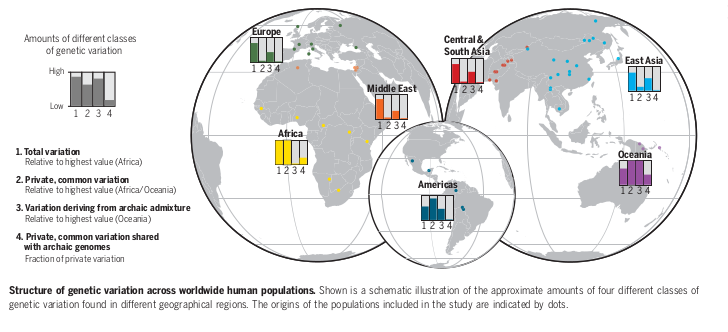
\includegraphics[width=1\textwidth]{Fig/HGDP.png}
\decoRule
\caption{}
\label{fig:HGDP}
\end{figure}

\section{Mitochondrial Genomes}
\subsection{Structure and function of mitochodria}
Mitochondria are a membrane-bound organelle present in the cytoplasm of all eukaryotic cells. They are responsible for producing Adenosine triphosphate (ATP), the main energy currency of the cell.
Mitochondria are typically round to oval in shape and range in size from 0.5 to 10 $\mu$m. In addition to producing energy, mitochondria store calcium for cell signaling activities, generate heat, and mediate cell growth and death.
Mitochondria are unlike other cellular o.<rganelles in that they have two distinct membranes and a unique genome and reproduce by binary fission. 
The outer mitochondrial membrane is freely permeable to small molecules and contains special channels capable of transporting large molecules. 
In contrast, the inner membrane is far less permeable, allowing only very small molecules to cross into the gel-like matrix that makes up the organelle’s central mass. 
The matrix contains the DNA of the mitochondrial genome (mtDNA) and the enzymes of the tricarboxylic acid (TCA) cycle (also known as the Krebs cycle), which metabolizes nutrients into by-products the mitochondrion can use for energy production. (Figure \ref{fig:Mitochondrial Function}) (\cite{friedman2014mitochondrial})

\subsection{Mitochondrial genome}
Mitochondrial DNA (mtDNA) is a double-stranded molecule of 16.6 kb. The two strands of mtDNA differ in their base composition, with one being rich in guanines, making it possible to separate a heavy (H) and a light (L) strand. The mtDNA contains one longer noncoding region (NCR) also referred to as the control region. DNA polymerase γ (POLγ) is the replicative polymerase in mitochondria. 
The circular genome contains 13 protein‐encoding sequences corresponding to subunits ND1‐6, including ND4 and ND4L, of respiratory complex I, catalytic subunits cytochrome c oxidase subunit I-III (CO1-3) of respiratory complex IV, subunits adenosine triphos-phate 6 (ATP6) and ATP8 of F1F0 ATPase, and cytochrome B of respiratory complex III. 
The remaining genes encode 22 tRNAs and 12, and 16S rRNAs. (Figure \ref{fig:Mitochondrial Genome}, \cite{stefano2016mitochondrial, garone2018mitochondrial})\\

Each human cell contains thousands of copies of mtDNA. At birth these are usually all identical (homoplasmy). Through life mutations can occur in one mtDNA and its descendants creating genetic variability of mitochondrial DNA within the same cell (heteroplasmy). Some of these mutations might be deleterious, therefore individuals with mitochondrial disorders resulting from mutation of mtDNA may harbor a mixture of mutated and wild type mtDNA within each cell. 

In many organisms, the mitochondrial genome is inherited maternally. This is because the mother’s egg cell donates the majority of cytoplasm to the embryo, and mitochondria inherited from the father’s sperm are usually destroyed but paternal mitochondrial DNA (mtDNA) transmission may coexist with maternal transmission of mtDNA. In a study on a family with mitochondrial disorders it was found that there was a high level of heteroplasmy due to paternally transmission (\cite{luo2018biparental}). 

\begin{figure}[H]
\centering
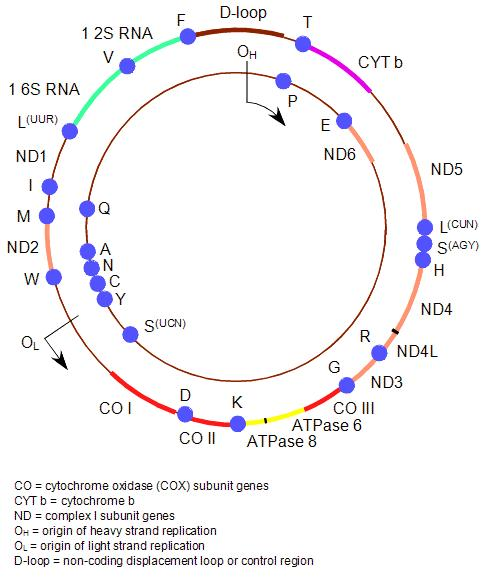
\includegraphics[width=0.7\textwidth]{Fig/mitogenome.jpg}
\decoRule
\caption{\textbf{Mitochondrial Genome}}
\label{fig:Mitochondrial Genome}
\end{figure}

\begin{figure}[H]
\centering
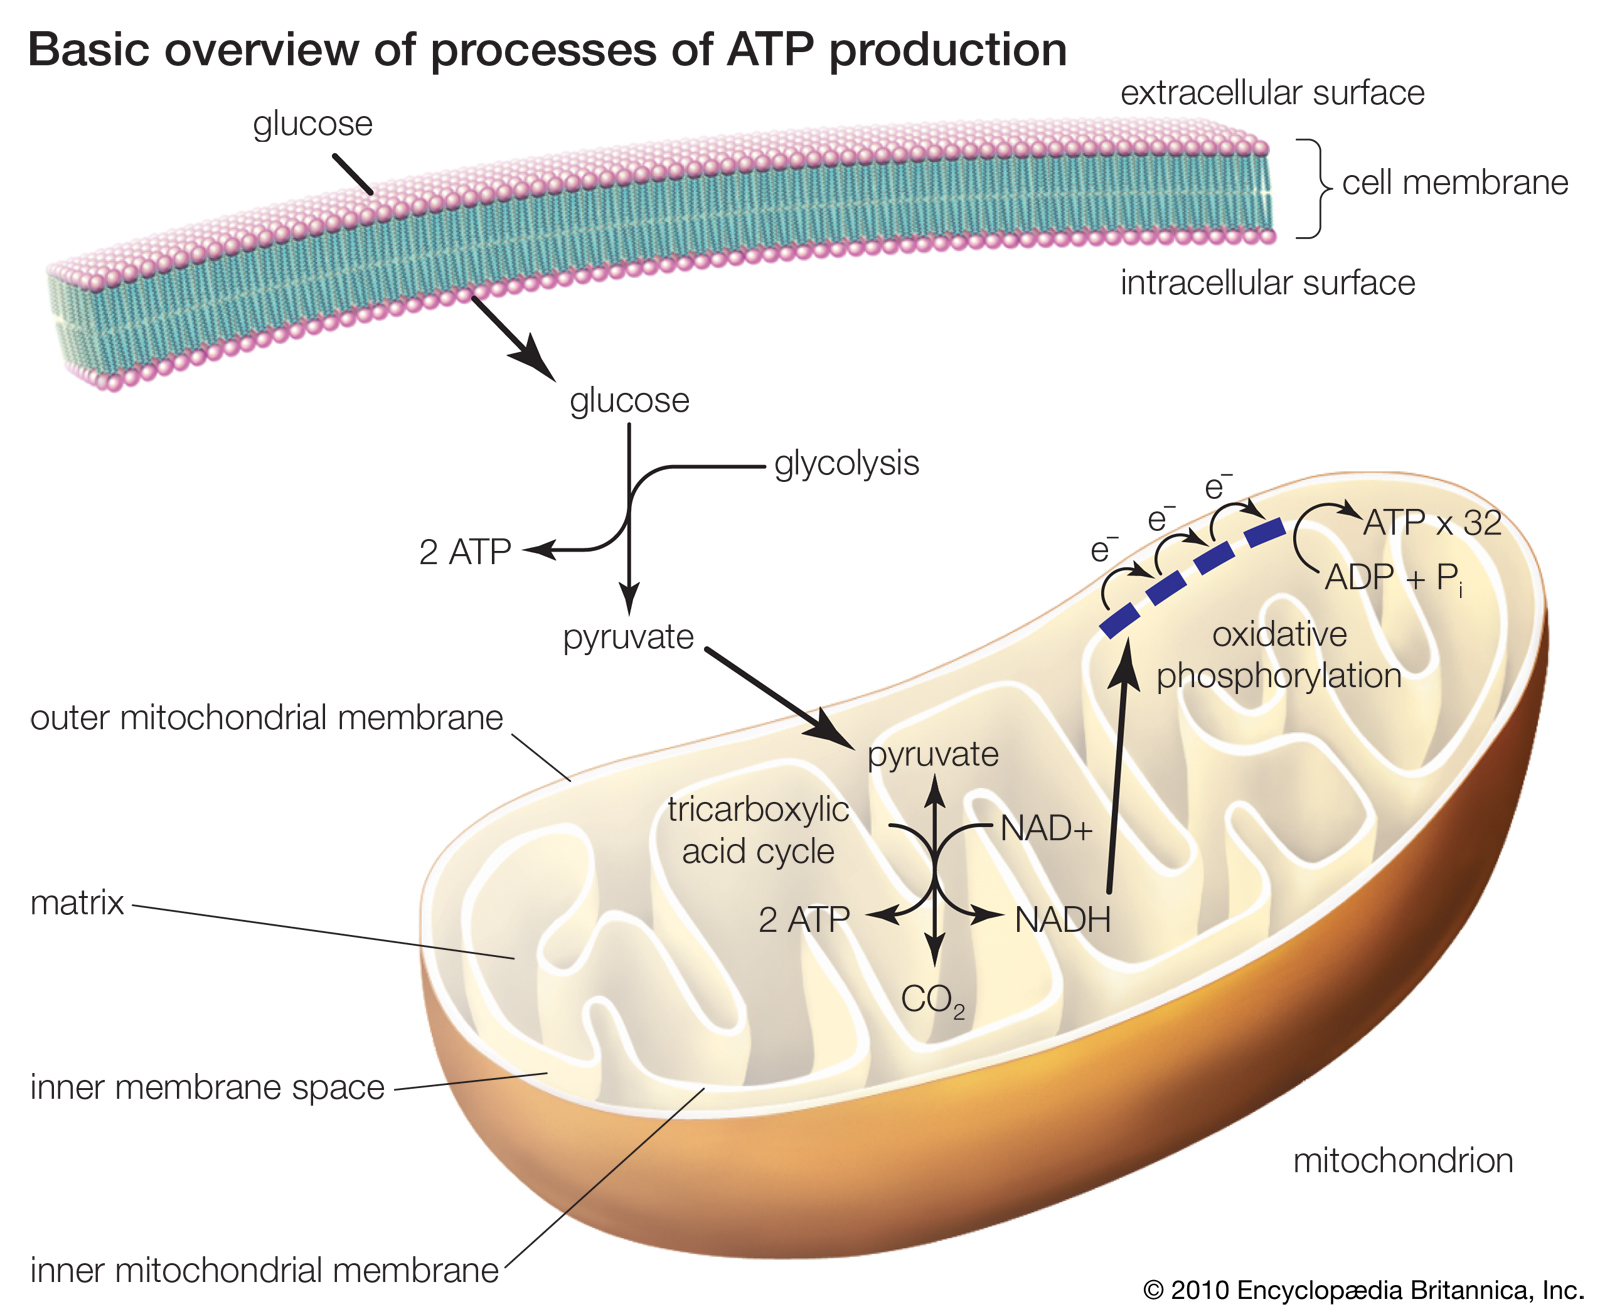
\includegraphics[width=0.7\textwidth]{Fig/processes-production-ATP-glycolysis-tricarboxylic-acid-cycle.jpg}
\decoRule
\caption{\textbf{Mitochondrial Function}}
\label{fig:Mitochondrial Function}
\end{figure}


\newline

\section{Expression of nuclear genes product in the mitochondria}
Not all the process taking place in mitochondria are controlled by mtDNA, in fact more than 1000 nuclear genes encode mitochondrial proteins.
Important mitochondrial mechanisms controlled by nuclear genes include disorders of mtDNA maintenance (mtDNA depletion or secondary pathogenic mtDNA variants), enzymes for lipid or cofactor biosynthesis (\textit{TAZ}), genes encoding factors for mitochondrial protein synthesis like the mitoribosomes encoded by \textit{MRPS22} (\cite{caggese1999identification, chinnery2014mitochondrial}). 
Most nuclear genes encode factors involved in the assembly of the complexes of the respiratory chain, like \textit{COX} genes, involved in stability and assembly of the respiratory complex.


\section{Mitochondrial Diseases}
Mitochondrial diseases are a clinically heterogeneous group of disorders that arise as a result of dysfunction of
the mitochondrial respiratory chain.
Single-cell studies and cybrid-cell studies have shown that the proportion of mutated mtDNA must exceed a critical threshold level before a cell expresses a biochemical abnormality of the mitochondrial respiratory chain (the threshold effect). The percentage level of mutated mtDNA may vary among individuals within the same family, and also among organs and tissues within the same individual (\cite{chinnery2014mitochondrial, thorburn2017mitochondrial}). 
While some mitochondrial disorders only affect a single organ (for example the eye in Leber hereditary optic neuropathy LHON), many involve multiple organ systems and often present with prominent neurologic and myopathic features , like Leigh syndrome.
Leigh syndrome (also called Leigh disease or subacute necrotizing
encephalomyelopathy) is a rare inherited neurometabolic disorder
and affects the central nervous system. 
Genetically, alterations or mutations of the mitochondrial respiratory enzyme complex or pyruvate dehydrogenase complex are believed to be responsible for the development of Leigh syndrome.
Brainstem dysfunction manifests as respiratory symptoms and abnormalities in swallowing, ophthalmology, and thermoregulation. 
The neurologic manifestations may begin in infancy or early
childhood, progressively worsen, and eventually lead to death in
early childhood ; Leigh syndrome can also occur at any age, including adolescence or adulthood.
(\cite{chang2020meta})


\section{Genetic causes of miscarriages}
Inefficiency in reproductive processes is known in humans. The prevalence of a miscarriage has been estimated to be between 10 and 15\% of all pregnancies, with the majority of these occurring in the first trimester of pregnancy.
Miscarriage is defined as the spontaneous termination of a pregnancy before 24 weeks of gestation.(\cite{larsen2013new , goddijn2000genetic}).
Miscarriages can occur for medicals or genetics causes. The most common medicals causes are TORCH infections, hypothyroidism,  diabetes and  uterine  anatomical  abnormalities . (\cite{najafi2019chromosomal}) . Among the genetic causes, chromosomal abnormalities are the major factor underlying early miscarriage and the most common are chromosomal aneuploidies such as trisomies or deletions of large chromosomal chunks (\cite{zhang2009genetic}) and can occur during mitosis in the oocytes or in sperms. Miscarriages can also have non random genetic causes like small mutations (SNPs and indels), both de-novo or inherited from parents (\cite{larsen2013new}).

\subsection{Mitochondrial diseases in miscarriages}

As far as genetic causes are concerned, it is important to remember the contribution of mitochondrial DNA in human reproduction inefficiency. 
Structural, spatial and genetic dysfunctions that affect the capacity of mitochondria to produce ATP by oxidative phosphorylation could have pleiotropic affects on early human development that may include the normality of spindle organization and chromosomal segregation. Mitochondrial dysfunctions that contribute to the activation of apoptosis may be a cause of human oocyte wastage and early embryo demise (\cite{van2004mitochondria}).
Mitochondrial dysfunction in the oocyte may be a critical determinant of the developmental competence of an early human embryo. Mitochondrial dysfunctions affecting ATP production during early developmental stages may be lethal for the embryo, even if only a portion of the mitochondria are dysfunctioning (\cite{karaa2019effects ,kaare2009mitochondrial}). Consequently, it is possible that some mtDNA mutations cause developmental arrest already before the pregnancy is clinically recognized (\cite{van2004mitochondria}). A fundamental role in mitochondrial diseases is played by homoplasmy/heteroplasmy level.
Homoplasmy for a severe pathogenic mtDNA mutation is rarely observed, presumably because of embryo lethality. 
Although a homoplasmic tRNA mutation has been reported in a family with six neonatal deaths and a miscarriage (\cite{mcfarland2002multiple}), mitochondrial mutations for diseases such as mitochondrial encephalopathy with lactic acidosis and stroke-like episodes (MELAS) and myoclonic epilepsy and ragged-red fibers (MERRF) are heteroplasmic, and homoplasmic mutations causing these syndromes would probably cause fetal demise (\cite{van2004mitochondria}).


\section{Project GREP}
The work I have done during my thesis is part of the project \textit{Genomics of REcurrent Pregnancy loss (GREP)} lead by the Institute of Genetics and Biophysics of the National Research Council in collaboration with the University of Napoli Federico II, and several other partners in Italy, United Kingdom, Malaysia, Pakistan, and Australia.  

GREP aims to identify genetic variants likely to cause PL not seen by current diagnostic tools (mainly comparative genomic hybridization), either because of the size or because they are located in non-coding regions not considered in medical diagnostics. The main objective of GREP is to build a predictive model that integrates genomic variation and functional annotations, based on the analysis of whole-genome sequences of miscarried embryos.\\

\chapter{Aim of the project }

in particolare mi sono occupata del dna mitocondriale 
lo scopo della mia tesi  e' 
objectives 
analizzare genoma mitocondriale di 10 embrioni di aborti spontanei per /study embryonic mitochondrial sequences from recurrent miscarriages in humans.: 
- characterize variabilita' mitocondriale 
- identify variants potentially detrimental 
- identify genes potentially involved



\chapter{Results}
%%%%%%%%%%%%%%%%%%%%%%%%%%%%%%%%%%%%%%%%%%%%%%%%%%%%%%%%%%%
%  Section 
%%%%%%%%%%%%%%%%%%%%%%%%%%%%%%%%%%%%%%%%%%%%%%%%%%%%%%%%%%%
\section{Description of the data set}
Data consist of eleven samples of genomics DNA of embryos from miscarriages of which 64\% are first pregnancy loss and 36\% are recurrent pregnancy loss.\\ 
A pregnancy loss is defined as the spontaneous demise of a pregnancy before the foetus reaches viability. The term therefore includes all pregnancy losses from the time of conception until 24 weeks of gestation.Recurrent pregnancy loss (RPL) is defined as the loss of two or more pregnancies.There has been significant debate in the literature and in the Guideline Development Group (GDG), on the definition of RPL and, more specifically, the extent to which this definition needs to be extended or constricted based on the number of losses and whether these are consecutive or not.
The exact prevalence of RPL is difficult to estimate, but most studies report that RPL affects 1–2\% of women. (\cite{eshre2018eshre})\\
%info embryos mother
The mothers of the embryos are mostly of European origin (87\%) and their median age at the date of collection was 36.7 years (sd=5.99), with no significant difference between first and recurrent cases. For the mothers of the embryos medical records report no major comorbidities. Median body mass index is within the range of normal weight (22.03, s.d.=4.26) and comparable between first and recurrent cases, as well as comparable to a group of control women. Similarly, menarche age is comparable among first, recurrent miscarriages, and controls.The recruited mothers of the embryos were in the range of healthy adult individuals.  \\
%FORSE NEI METODI  
Sequencing was done through a service provider (Macrogen s.r.l). In particular, libraries for sequencing were prepared using the Illumina TruSeq DNA PCR-free Library (insert size 350bp) and samples were sequenced at 30X mapped (~110Gb) 150bp PE on HiSeqX. Data were released in as fastq files. 
Alignment with reference Reads in the fastq file were aligned against the reference genome GRChg38.p12 (\cite{rosenbloom2015ucsc}) using \textsc{bwa} and \textsc{samtools}. \textsc{bwa}

%%%%%%%%%%%%%%%%%%%%%%%%%%%%%%%%%%%%%%%%%%%%%%%%%%%%%%%%%%%
%  Section 
%%%%%%%%%%%%%%%%%%%%%%%%%%%%%%%%%%%%%%%%%%%%%%%%%%%%%%%%%%%

\section{Characterization of variants in the mitochondrial DNA}




\subsection{Identification of variants}
The sequencing process produces sequence data in the \gls{fastq} format, i.e. the raw sequence data that I used to perform the variant calling analysis on high performance computing machines. %Figure \ref{fig:align-ref-vc} provides an overview of the pipeline used in this study.\newline
The variant calling is the process of identification of variants from sequence data, where variants are chunks of sequence that differ from the reference genome. Genetic variants are classified as single nucleotide variants (SNVs), small insertions and deletions (indels), and structural variants (SVs, large genomic rearrangements). (Figure \ref{Fig:variantCalling})

\begin{figure}[H]
\centering
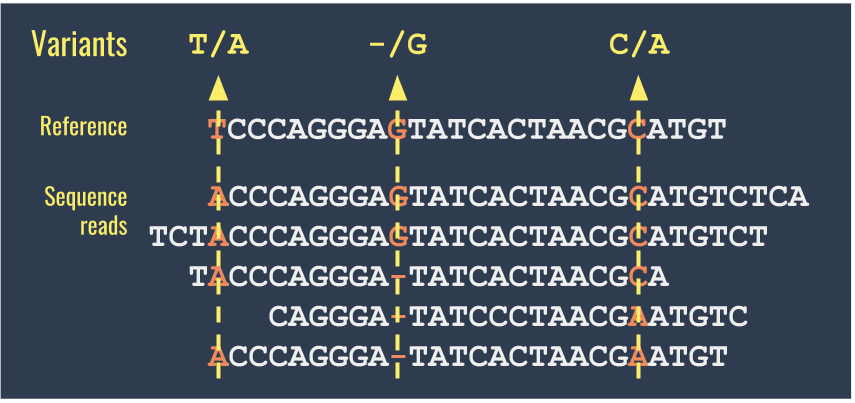
\includegraphics[width=0.7\textwidth]{Fig/variantCalling.png}
\decoRule
\caption{\textbf{Variant calling} is the process of identifying genetic variants. First, sequence reads from one individual are aligned against the reference genome, then variable sites are identified as the ones where the sequence differs from the reference genome.} 
\label{fig:variantCalling}
\end{figure}



The first step in variant calling is the \textbf{alignment} of the raw sequence data in form of reads against the most recent version of the human reference Genome (GRChg38.p12, \cite{rosenbloom2015ucsc}) using \textsc{bwa-mem} (\cite{li2013aligning}) and \textsc{samtools} (\cite{li2009sequence}). The alignment produces files in the bam format that provide information on the quality of the alignment and enable some quality controls.  In our data set the majority of the reads were correctly aligned to the reference genome. 

Before proceeding to the next step I used \textsc{sambamba} (\cite{tarasov2015sambamba}) to \textbf{refine} the data and remove PCR duplicates, i.e. reads that came from the same DNA fragment that bias variant detection through increased homozygosity.\newline

I used the refined bam file to perform \textbf{variant calling} using \textsc{mity} (\cite{puttick2019mity}) that is based on the \textsc{freebayes} algorithm (\cite{garrison2012haplotype}). Variant calling produces data in the vcf format. 

The final step is a second round of \textbf{refining} that includes three steps. 
\begin{itemize}
    \item I used \textsc{vcffilter} (\cite{vcflib}) to filter variants for \gls{quality score}(QUAL)>30. The QUAL is an estimate of how likely it is to observe a call by chance, and a value of 30 corresponds to 1\% probability of having an incorrect genotype.
    \item I used \textsc{vt} (\cite{tan2015unified}) to do the normalization that consist of two parts: parsimony and left alignment. Parsimony is the representation of a variant in as few nucleotides as possible without reducing the length of any allele to 0. Left alignment is the shift of the start position of a variant to the left till it is no longer possible to do so (Figure \ref{fig:vtNorm}) (\cite{tan2015unified}).
    \item I used \textsc{vt} to deconstruct multiallelic variants in a VCF to allow for allelic comparisons between call sets
\end{itemize}

\begin{figure}[H]
\centering
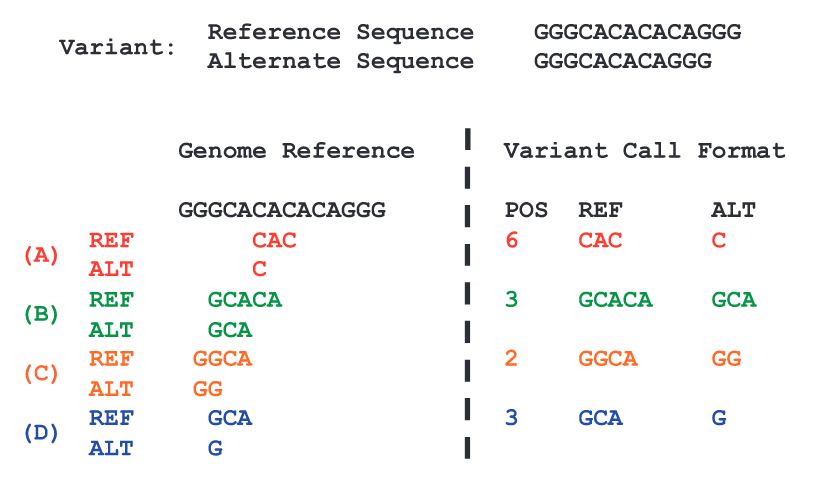
\includegraphics[width=0.65\textwidth]{Fig/vtNormalizeTan.png}
\decoRule
\caption{\textbf{Example  of  VCF  entries  representing  the  same  variant.} \textit{ Adapted from \cite{tan2015unified}}. Left  panel aligns each allele to the reference genome, and the right panel represents thevariant in VCF. (A) is not left-aligned (B) is neither left-aligned nor parsimonious, (C) is not parsimonious and (D) is normalized}
\label{fig:vtNorm}
\end{figure}

\begin{figure}[H]
\centering
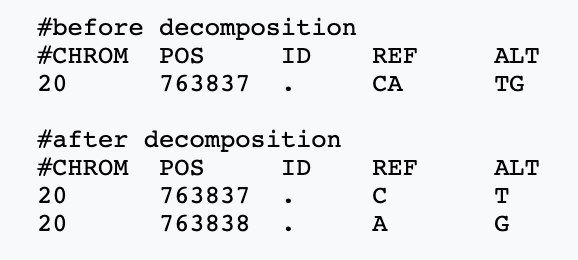
\includegraphics[width=0.5\textwidth]{Fig/vtDecompose.png}
\decoRule
\caption{\textbf{Decomposes biallelic clumped variant} for allelic comparisons between call sets} \textit{ Adapted from \cite{tan2015unified}}. 
\label{fig:vtDecomp}
\end{figure}

Overall, the variant calling with \textsc{mity} identified 276 unique variable sites of which 44 are in the D-Loop (positions 309-566) that is more variable than the rest of the mitochondrial DNA as expected (\cite{chinnery2014mitochondrial}). In particular there is one variable sites every 5.8 bp in the D-loop \textit{versus} 70.3 bp in the rest of DNA.\\

Per each sample, the number of variable sites vary between 22 and 103 (Table \ref{tab:stats_variantcalling}). On average, the majority (90\%) of the variants is Single Nuclotide Variants. The other types of variants are indels.\\

{\begin{table}
\caption{Variant classes count per sample}
\label{tab:stats_variantcalling}
\centering
\begin{tabular}{1 1 1 1 1 1}
\toprule
\tabhead{ID} & \tabhead{SNV} & \tabhead{InDels} & \tabhead{}    \\
\midrule
AS006 & 22 & 5  \\
AS030 & 18 & 4  \\
AS036 & 28 & 1  \\
AS054 & 94 & 9   \\
AS064 & 17 & 3   \\
AS065 & 61 & 5  \\
AS074 & 22 & 2  \\
AS087 & 46 & 1  \\
AS090 & 41 & 3   \\
AS093 & 45 & 1  \\
AS094 & 47 & 7   \\
\bottomrule\\
\end{tabular}
\end{table}
}
 

%%%%%%%%%%%%%%%%%%%%%%%%%%%%%%%%%%%%%
\subsection{Functional annotations of variants}

The  Variant Effect Predictor (VEP) software determines the effect of variants (SNPs, insertions, deletions, CNVs or structural variants) on genes, transcripts, and protein sequence, as well as regulatory regions (\cite{mclaren2016ensembl}). I run VEP on the vcf files obtained from the variant calling

{\small
\begin{sidewaystable}
\caption{Table of Consequences}
\label{tab:csqVEP}
\centering
\begin{adjustbox}{width=1\textwidth}
\begin{tabular}{c c c c}
\toprule
\tabhead{SO term} & \tabhead{SO description} & \tabhead{SO accession} & \tabhead{Impact} \\
\midrule
transcript ablation & A feature ablation whereby the deleted region includes a transcript feature & SO:0001893 & HIGH \\
splice acceptor variant & A splice variant that changes the 2 base region at the 3' end of an intron & SO:0001574 & HIGH \\
splice donor variant & A splice variant that changes the 2 base region at the 5' end of an intron & SO:0001575 & HIGH \\
stop gained & A sequence variant whereby at least one base of a codon is changed, resulting in a premature stop codon, leading to a shortened transcript & SO:0001587 & HIGH \\
frameshift variant & A sequence variant which causes a disruption of the translational reading frame, because the number of nucleotides inserted or deleted is not a multiple of three & SO:0001589 & HIGH \\
stop lost & A sequence variant where at least one base of the terminator codon (stop) is changed, resulting in an elongated transcript & SO:0001578 & HIGH \\
start lost & A codon variant that changes at least one base of the canonical start codon & SO:0002012 & HIGH \\
transcript amplification & A feature amplification of a region containing a transcript & SO:0001889 & HIGH \\
inframe insertion & An inframe non synonymous variant that inserts bases into in the coding sequence & SO:0001821 & MODERATE \\
inframe deletion & An inframe non synonymous variant that deletes bases from the coding sequence & SO:0001822 & MODERATE \\
missense variant & A sequence variant, that changes one or more bases, resulting in a different amino acid sequence but where the length is preserved & SO:0001583 & MODERATE \\
protein altering variant & A sequence variant which is predicted to change the protein encoded in the coding sequence & SO:0001818 & MODERATE \\
splice region variant & A sequence variant in which a change has occurred within the region of the splice site, either within 1-3 bases of the exon or 3-8 bases of the intron & SO:0001630 & LOW \\
incomplete terminal codon variant & A sequence variant where at least one base of the final codon of an incompletely annotated transcript is changed & SO:0001626 & LOW \\
start retained variant & A sequence variant where at least one base in the start codon is changed, but the start remains & SO:0002019 & LOW \\
stop retained variant & A sequence variant where at least one base in the terminator codon is changed, but the terminator remains & SO:0001567 & LOW \\
synonymous variant & A sequence variant where there is no resulting change to the encoded amino acid & SO:0001819 & LOW \\
coding sequence variant & A sequence variant that changes the coding sequence & SO:0001580 & MODIFIER \\
mature miRNA variant & A transcript variant located with the sequence of the mature miRNA & SO:0001620 & MODIFIER \\
5 prime UTR variant & A UTR variant of the 5' UTR & SO:0001623 & MODIFIER \\
3 prime UTR variant & A UTR variant of the 3' UTR & SO:0001624 & MODIFIER \\
non coding transcript exon variant & A sequence variant that changes non-coding exon sequence in a non-coding transcript & SO:0001792 & MODIFIER \\
intron variant & A transcript variant occurring within an intron & SO:0001627 & MODIFIER \\
NMD transcript variant & A variant in a transcript that is the target of NMD & SO:0001621 & MODIFIER \\
non coding transcript variant & A transcript variant of a non coding RNA gene & SO:0001619 & MODIFIER \\
upstream gene variant & A sequence variant located 5' of a gene & SO:0001631 & MODIFIER \\
downstream gene variant & A sequence variant located 3' of a gene & SO:0001632 & MODIFIER \\
TFBS ablation & A feature ablation whereby the deleted region includes a transcription factor binding site & SO:0001895 & MODIFIER \\
TFBS amplification & A feature amplification of a region containing a transcription factor binding site & SO:0001892 & MODIFIER \\
TF binding site variant & A sequence variant located within a transcription factor binding site & SO:0001782 & MODIFIER \\
regulatory region ablation & A feature ablation whereby the deleted region includes a regulatory region & SO:0001894 & MODERATE \\
regulatory region amplification & A feature amplification of a region containing a regulatory region & SO:0001891 & MODIFIER \\
feature elongation & A sequence variant that causes the extension of a genomic feature, with regard to the reference sequence & SO:0001907 & MODIFIER \\
regulatory region variant & A sequence variant located within a regulatory region & SO:0001566 & MODIFIER \\
feature truncation & A sequence variant that causes the reduction of a genomic feature, with regard to the reference sequence & SO:0001906 & MODIFIER \\
intergenic variant & A sequence variant located in the intergenic region, between genes & SO:0001628 & MODIFIER \\
\bottomrule\\
\end{tabular}
\end{adjustbox}
\end{sidewaystable}
}

Table \ref{tab:csqVEP} (adapted from \cite{mclaren2016ensembl}) describes the classification of the consequences in the Ensembl Variation data base.

%Variant classes 
The VEP software identifies 4 classes of variants (Figure \ref{fig:variantclass}), in which we distinguish deletion (n=6), insertion (n=30) and SNV (n=240).



\begin{figure}[h]
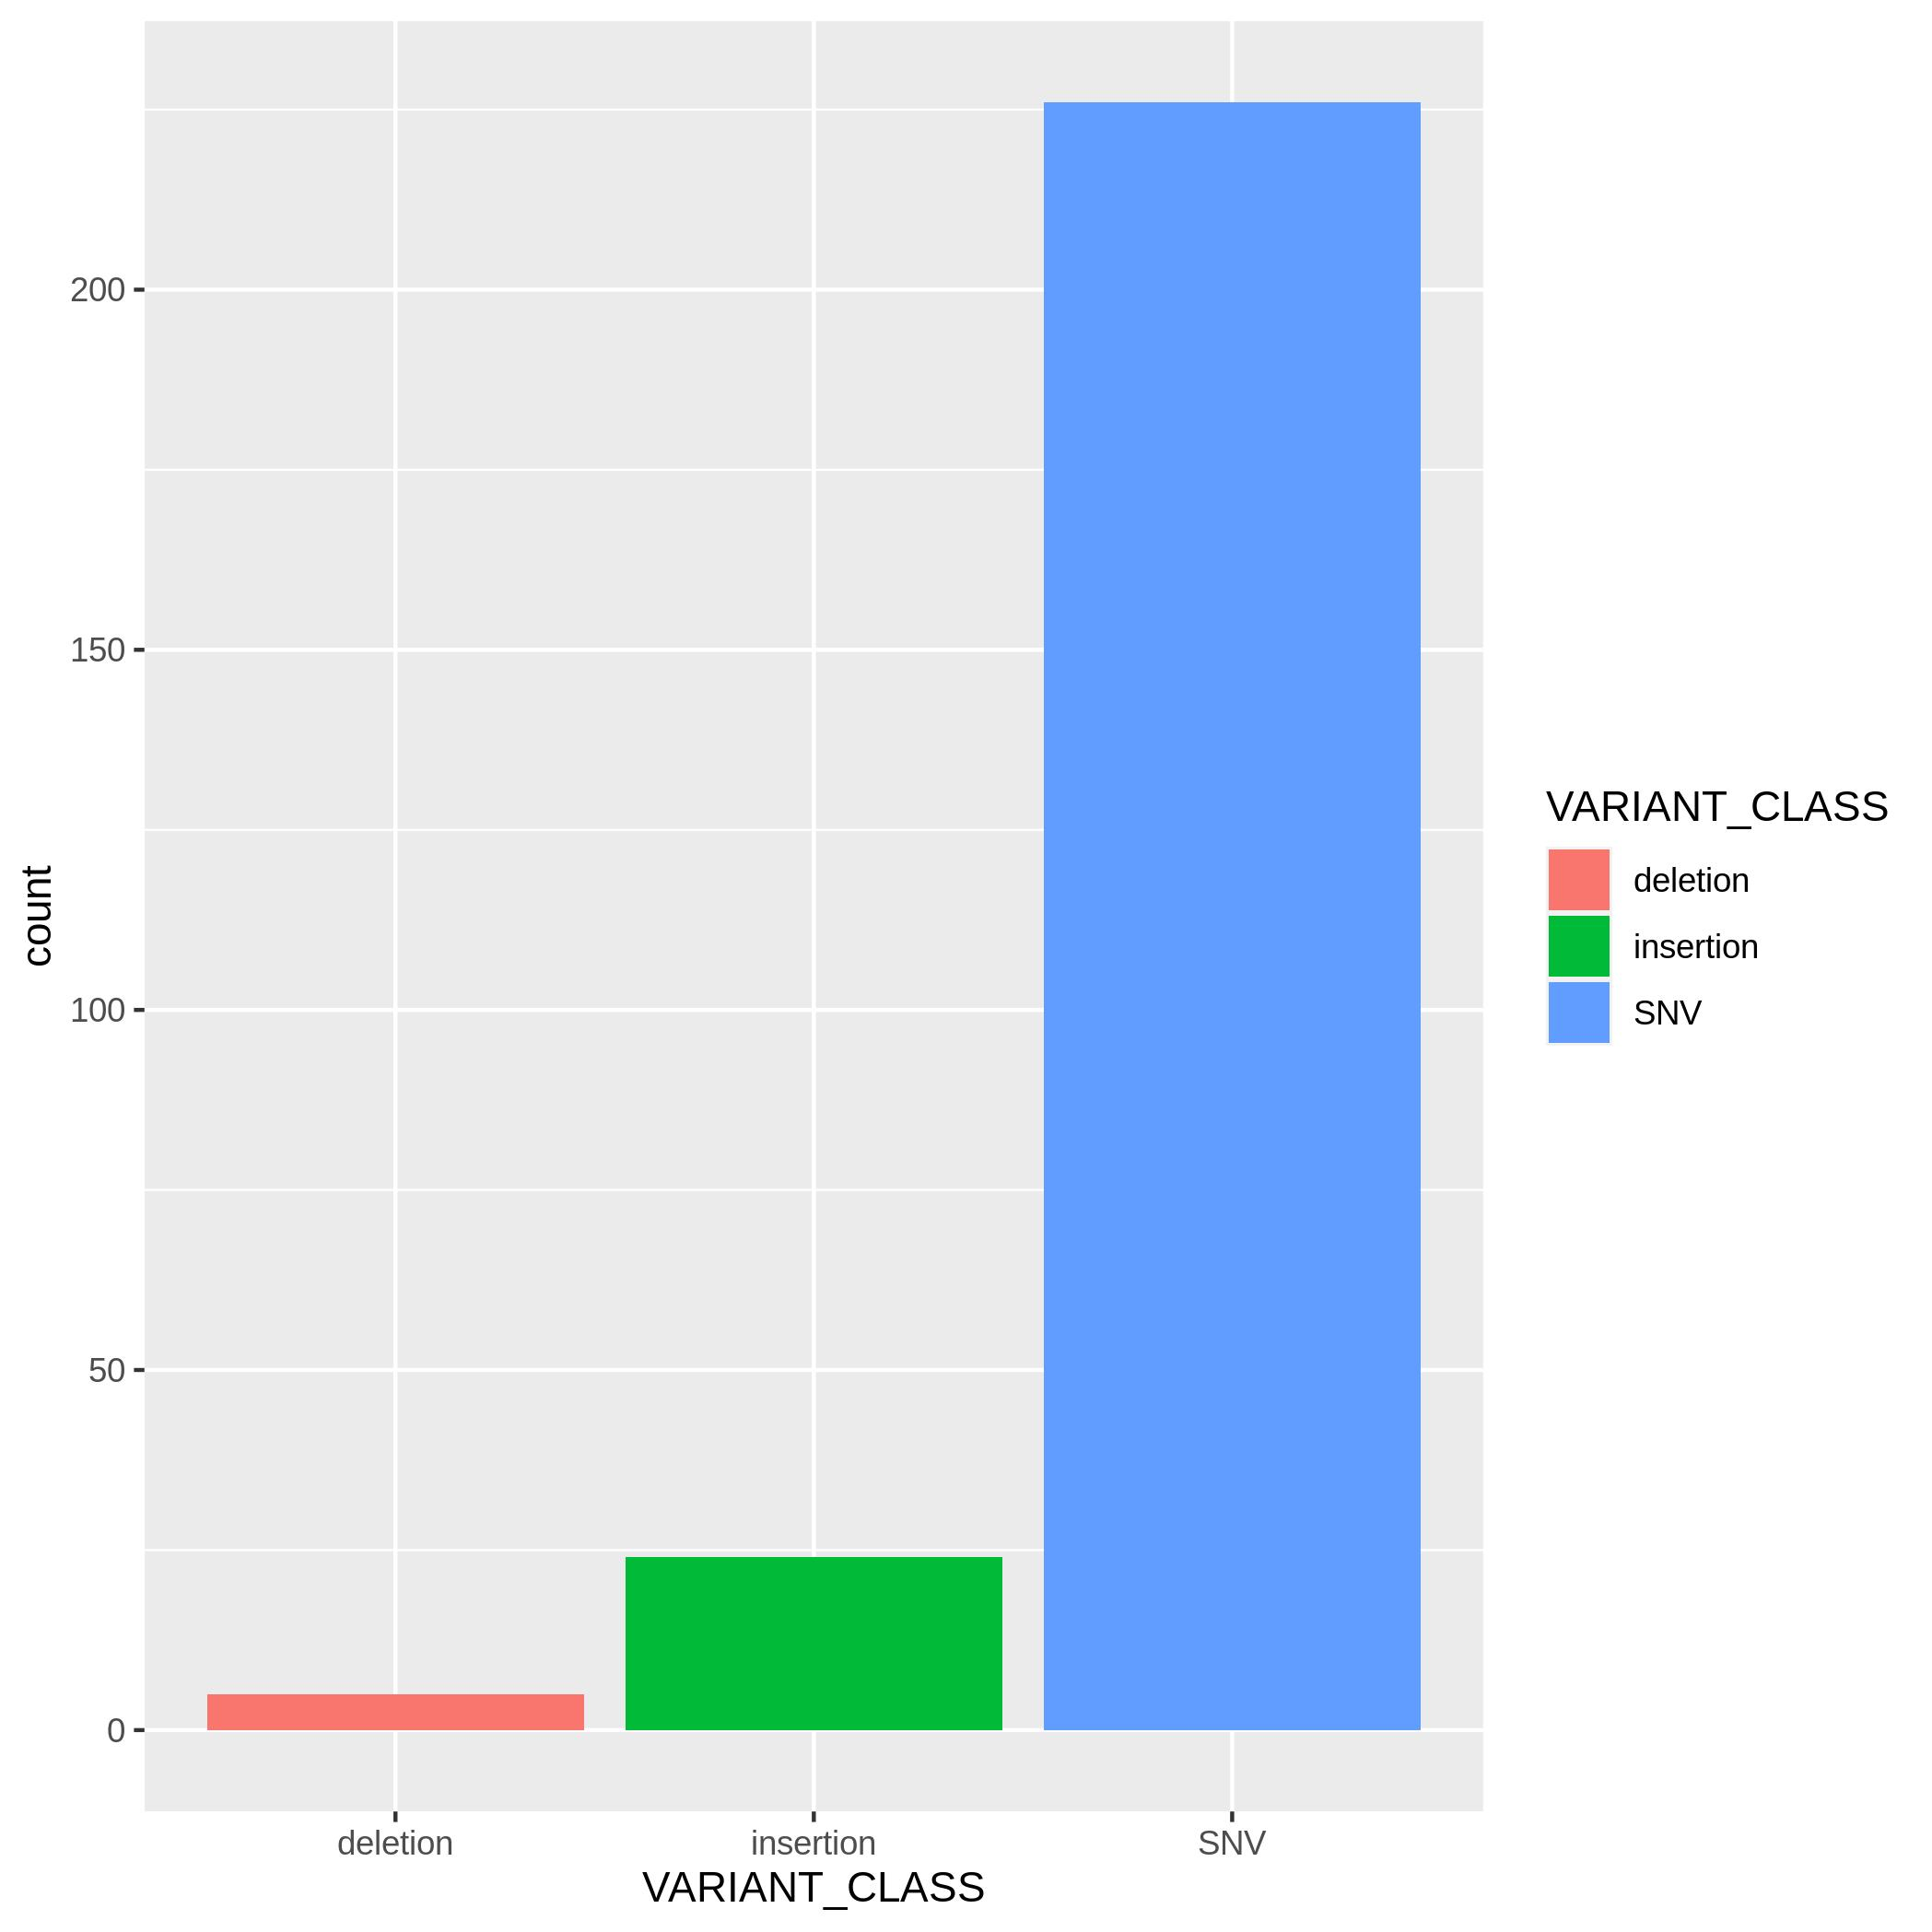
\includegraphics[width=8cm]{Fig/VC_vep_deco.jpg}
\caption{}
\label{fig:variantclass}
\end{figure}


%Most severe consequence
VEP identifies the most severe consequence for the given variants. In our DNA sequences VEP classifies the majority as upstream gene variants (112), 84 as synonymous variant, 46 as missense variant, and 34 are non coding transcript exon variant.


Among variants in the coding consequences there are synonymous and missense. Synonymous mutations on the DNA sequence results in the same amino acid, therefore they are considered of low impact. Missense variants are instead considered of high impact because their effect is to change the amino acid in the protein coded by the gene therefore, missense variants can alter the function of the protein. For the missense variants, VEP annotates also SIFT and PolyPhen scores. SIFT predicts whether an amino acid substitution affects protein function based on sequence homology and the physical properties of amino acids (\cite{ng2003sift}). The SIFT score ranges from 0.0 (deleterious) to 1.0 (tolerated). In my samples there are 21 variants defined as tolerated with low confidence, 13 deleterious with low confidence, 8 tolerated variants and 4 deleterous (Figure \ref{fig:siftpolyphen}).
 

The PolyPhen score predicts the possible impact of an amino acid substitution on the structure and function of a human protein \cite{adzhubei2013predicting}.The PolyPhen score ranges from 0.0 (tolerated) to 1.0 (deleterious). Variants with scores of 0.0 are predicted to be benign. Values closer to 1.0 are more confidently predicted to be deleterious. In my samples I find 28 benign variants, 15 probably damaging variants, 2 possibly damaging variants and 1 unknown (Figure \ref{fig:siftpolyphen}).\\


%figura 
\begin{figure}[h]
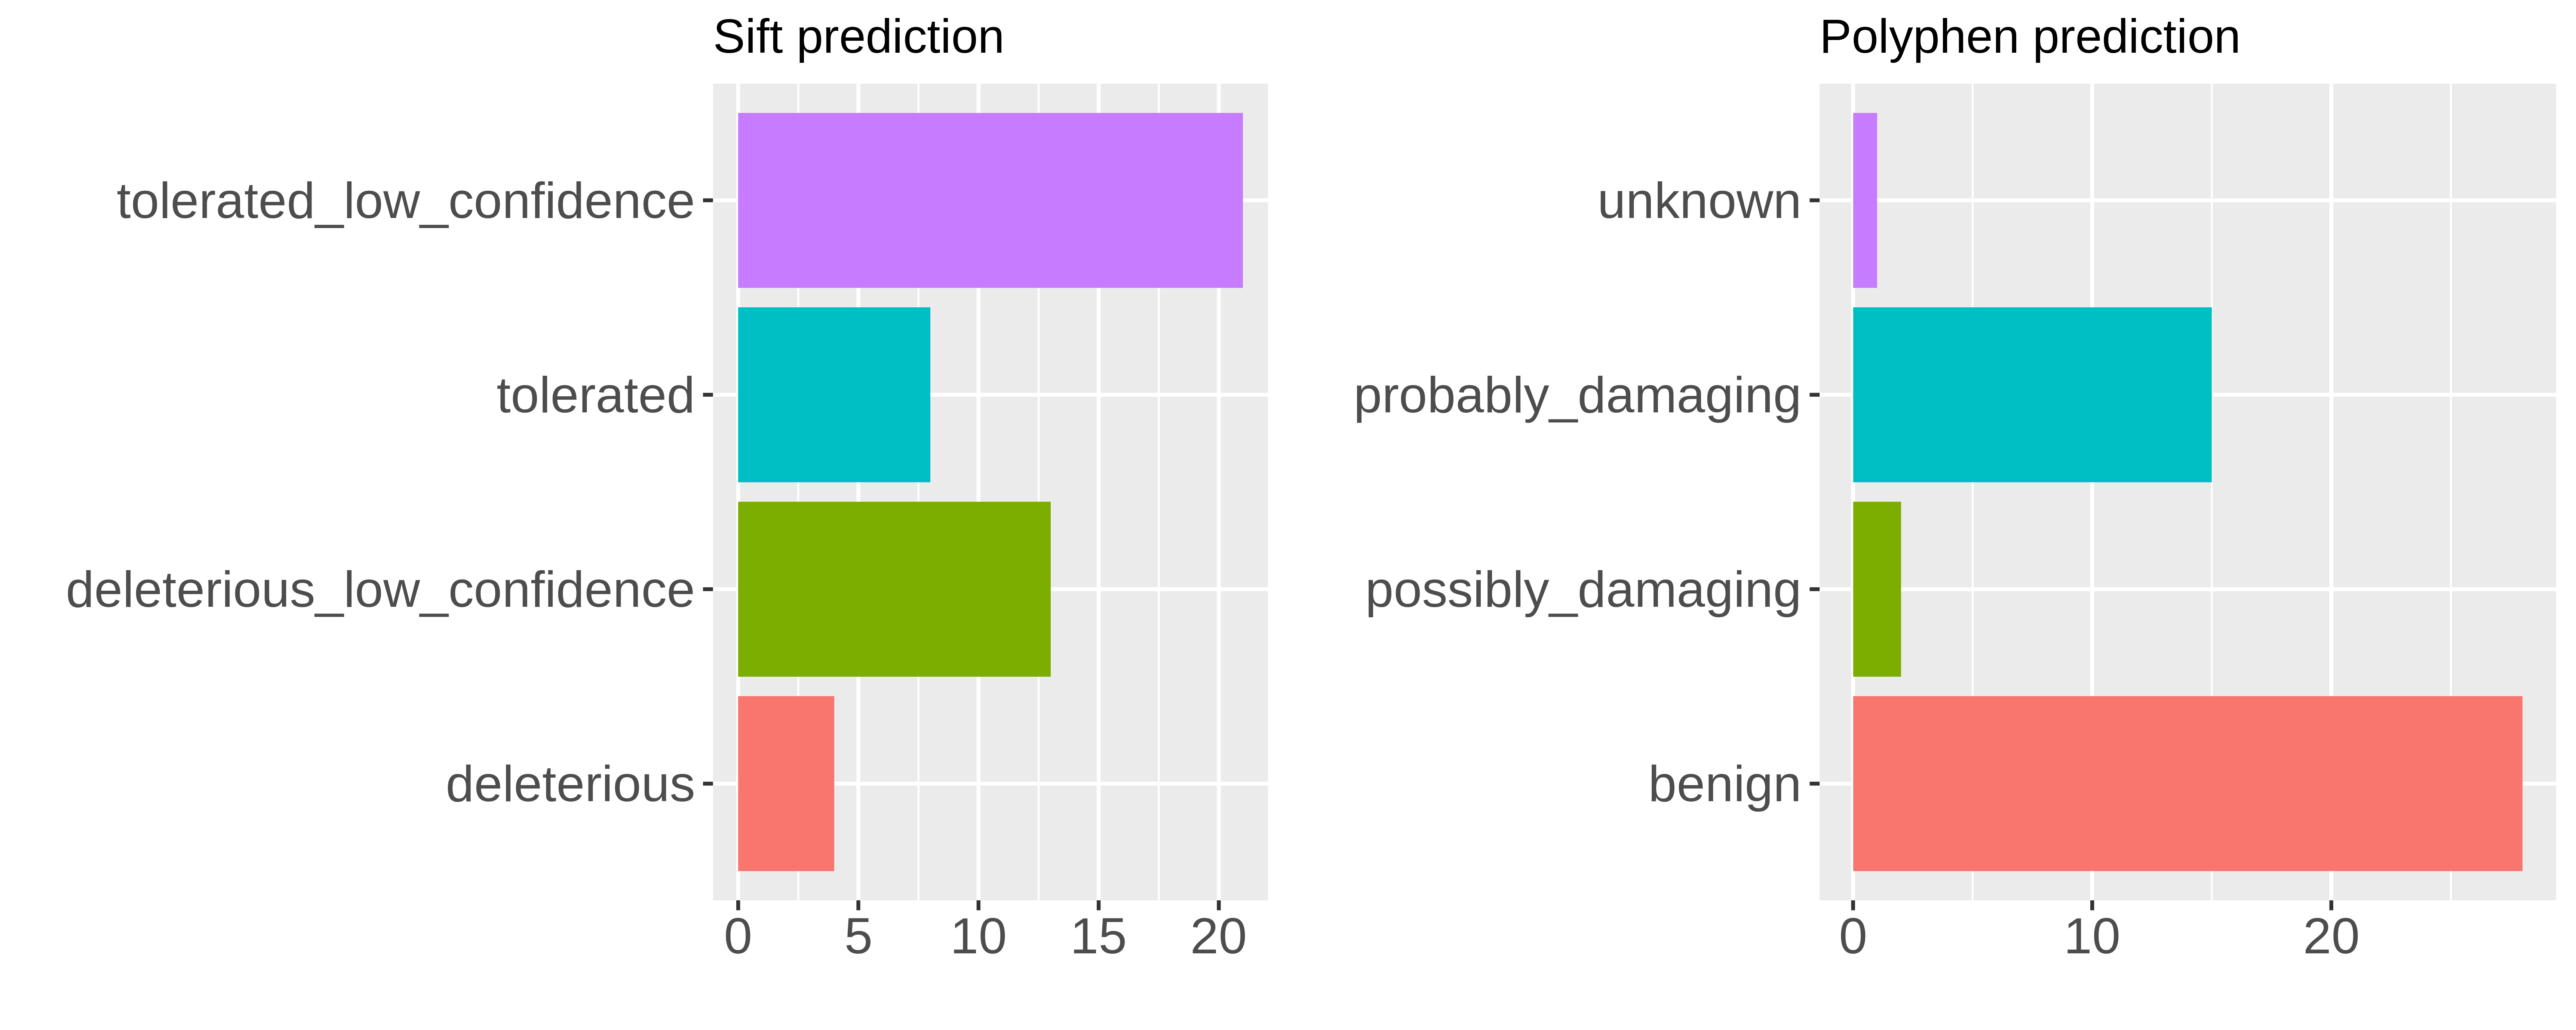
\includegraphics[width=\textwidth]{Fig/plots2.png}
\caption{Sift and Polyphen}
\label{fig:siftpolyphen}
\end{figure}\\


I have considered the 4 deleterious variants of SIFT described in Table \ref{tab:missense}. The variants are located at positions "5374" with PolyPhen  benign with a score of 0.253, "8668" with PolyPhen probably damaging with a score of 0.947, "14447" with PolyPhen possibly damaging with a score of 0.861 and at position "14556" with PolyPhen probably damaging with score 0.999. These variants are found in the \textit {MT-ND2}, \textit{MT-ATP6} and \textit{MT-ND6} genes\\ 
These four variants are shared by more than one sample, in particular the variant at position 14556 in the \textit{MT-ND6} gene is shared by 8 samples (Table \ref{tab:missenseDel0.genotypes}). \\

\textit{MT-ND2} is a mitochondrial gene coding for the NADH dehydrogenase 2 (ND2) protein.The ND2 protein is a subunit of NADH dehydrogenase (ubiquinone), which is located in the mitochondrial inner membrane and is the largest of the five complexes of the electron transport chain. (\cite{ncbi2016database})\\
\textit{MT-ATP6} (or ATP6) is a mitochondrial gene that encodes the ATP synthase Fo subunit 6 (or subunit/chain A).This subunit belongs to the Fo complex of the complex V. This enzyme is responsible for the final step of oxidative phosphorylation in the electron transport chain. (\cite{ncbi2016database})\\

\textit{MT-ND6} is a mitochondrial gene coding for the NADH-ubiquinone oxidoreductase chain 6 protein (ND6). The ND6 protein is a subunit of NADH dehydrogenase (ubiquinone), which is located in the mitochondrial inner membrane and is the largest of the five complexes of the electron transport chain.
 (\cite{ncbi2016database})\\


%rs non riportati

{\small
\begin{table}
\caption{Missense Variants}
\label{tab:missense}
\centering
\begin{adjustbox}{width=1\textwidth}
\begin{tabular}{c c c c c c c}
\toprule
\tabhead{Location chrM} & \tabhead{Variation Allele} & \tabhead{existing Variation} & \tabhead{Codons} & \tabhead{SYMBOL} & \tabhead{SIFT (score)} & \tabhead{PolyPhen (score)} \\
\midrule
5374 & T/C  & - & aTc/aCc & MT-ND2 & deleterious (0) &  benign (0.253)   \\%ENSG00000198763
8668 & T/C &  COSV62293167 & Tga/Cga & MT-ATP6 & deleterious (0)&      probably damaging (0.997)   \\ %ENSG00000198899
14447 & T/C & - & gAg/gGg & MT-ND6 & deleterious (0) &     possibly damaging (0.861) \\ %ENSG00000198695
14556 & A/C & - & Tgt/Ggt & MT-ND6 & deleterious (0) &      probably damaging (0.999)   \\ %ENSG00000198695
\bottomrule\\
\end{tabular}
\end{adjustbox}
\end{table}
}

Pathogenic variants of the mitochondrial gene \textit{MT-ND2} are known to cause mtDNA-associated Leigh syndrome, as are variants of \textit{MT-ATP6} and \textit{MT-ND6}. Abnormalities in mitochondrial energy generation result in neurodegenerative disorders like Leigh syndrome, which is characterized by an onset of symptoms between 12 months and three years of age. The symptoms frequently present themselves following a viral infection and include movement disorders and peripheral neuropathy, as well as hypotonia, spasticity and cerebellar ataxia. Roughly half of affected patients die of respiratory or cardiac failure by the age of three. Leigh syndrome is a maternally inherited disorder and its diagnosis is established through genetic testing of the aforementioned mitochondrial genes
(\cite{thorburn2017mitochondrial})


 


{\small
\begin{table}
\caption{missense.genotypes}
\label{tab:missenseDel0.genotypes}
\centering
\begin{tabular}{c c c c c c c}
\toprule
\tabhead{Sample ID} & \tabhead{5374} & \tabhead{8668} & \tabhead{14447} & \tabhead{14556}\\
\midrule 
AS006   &      0   &    0   &    0   &    1\\
AS030   &      0   &    0   &    0   &    0\\
AS036   &      1   &    0   &    1   &    1\\
AS054   &      1   &    1   &    1   &    1\\
AS064   &      0   &    0   &    0   &    1\\
AS065   &      0   &    0   &    1   &    0\\
AS074   &      0   &    0   &    0   &    0\\
AS087   &      1   &    0   &    0   &    1\\
AS090   &      0   &    0   &    1   &    1\\
AS093   &      1   &    1   &    1   &    1\\
AS094   &      1   &    0   &    1   &    1\\
TOTAL SHARED   &     5    &    2  &     6   &    8\\
\bottomrule\\
\end{tabular}
\end{table}
}



\section{Nuclear genes involved in mitochondrial process}

After exploring variation in the mitochondrial genome, I have analyzed variation in nuclear genes whose product are involved in mitochondrial processes. First I selectd these genes using gene ontology(GO). The GO database (\cite{ashburner2000gene}) is a collection of structured vocabularies, or ontologies, that describe and relate gene products in terms of their biological properties.
In GO I found 1,384 genes involved in mitochondrial process. 

I then run the \textsc{VEP} analysis to annotate the 766,845 variants found in the 1,384 genes that are presents in the ten genomes of the embryos and the results are summarized in Figure (\ref{fig:mostsevereconsequence}), stratified by four categories of impact: High, Modifier, Moderate, and Low.
The majority of variants (NUMERO ESATTO) are intronic with modifier impact. There are 6X variants with moderate effect and nine variants with high impact.  
Among the variants with high impact the most frequent type is splice acceptor, followed by splice donor and frameshift (Table \ref{tab:MostSevereConsequence}). 
 

\begin{figure}[h]
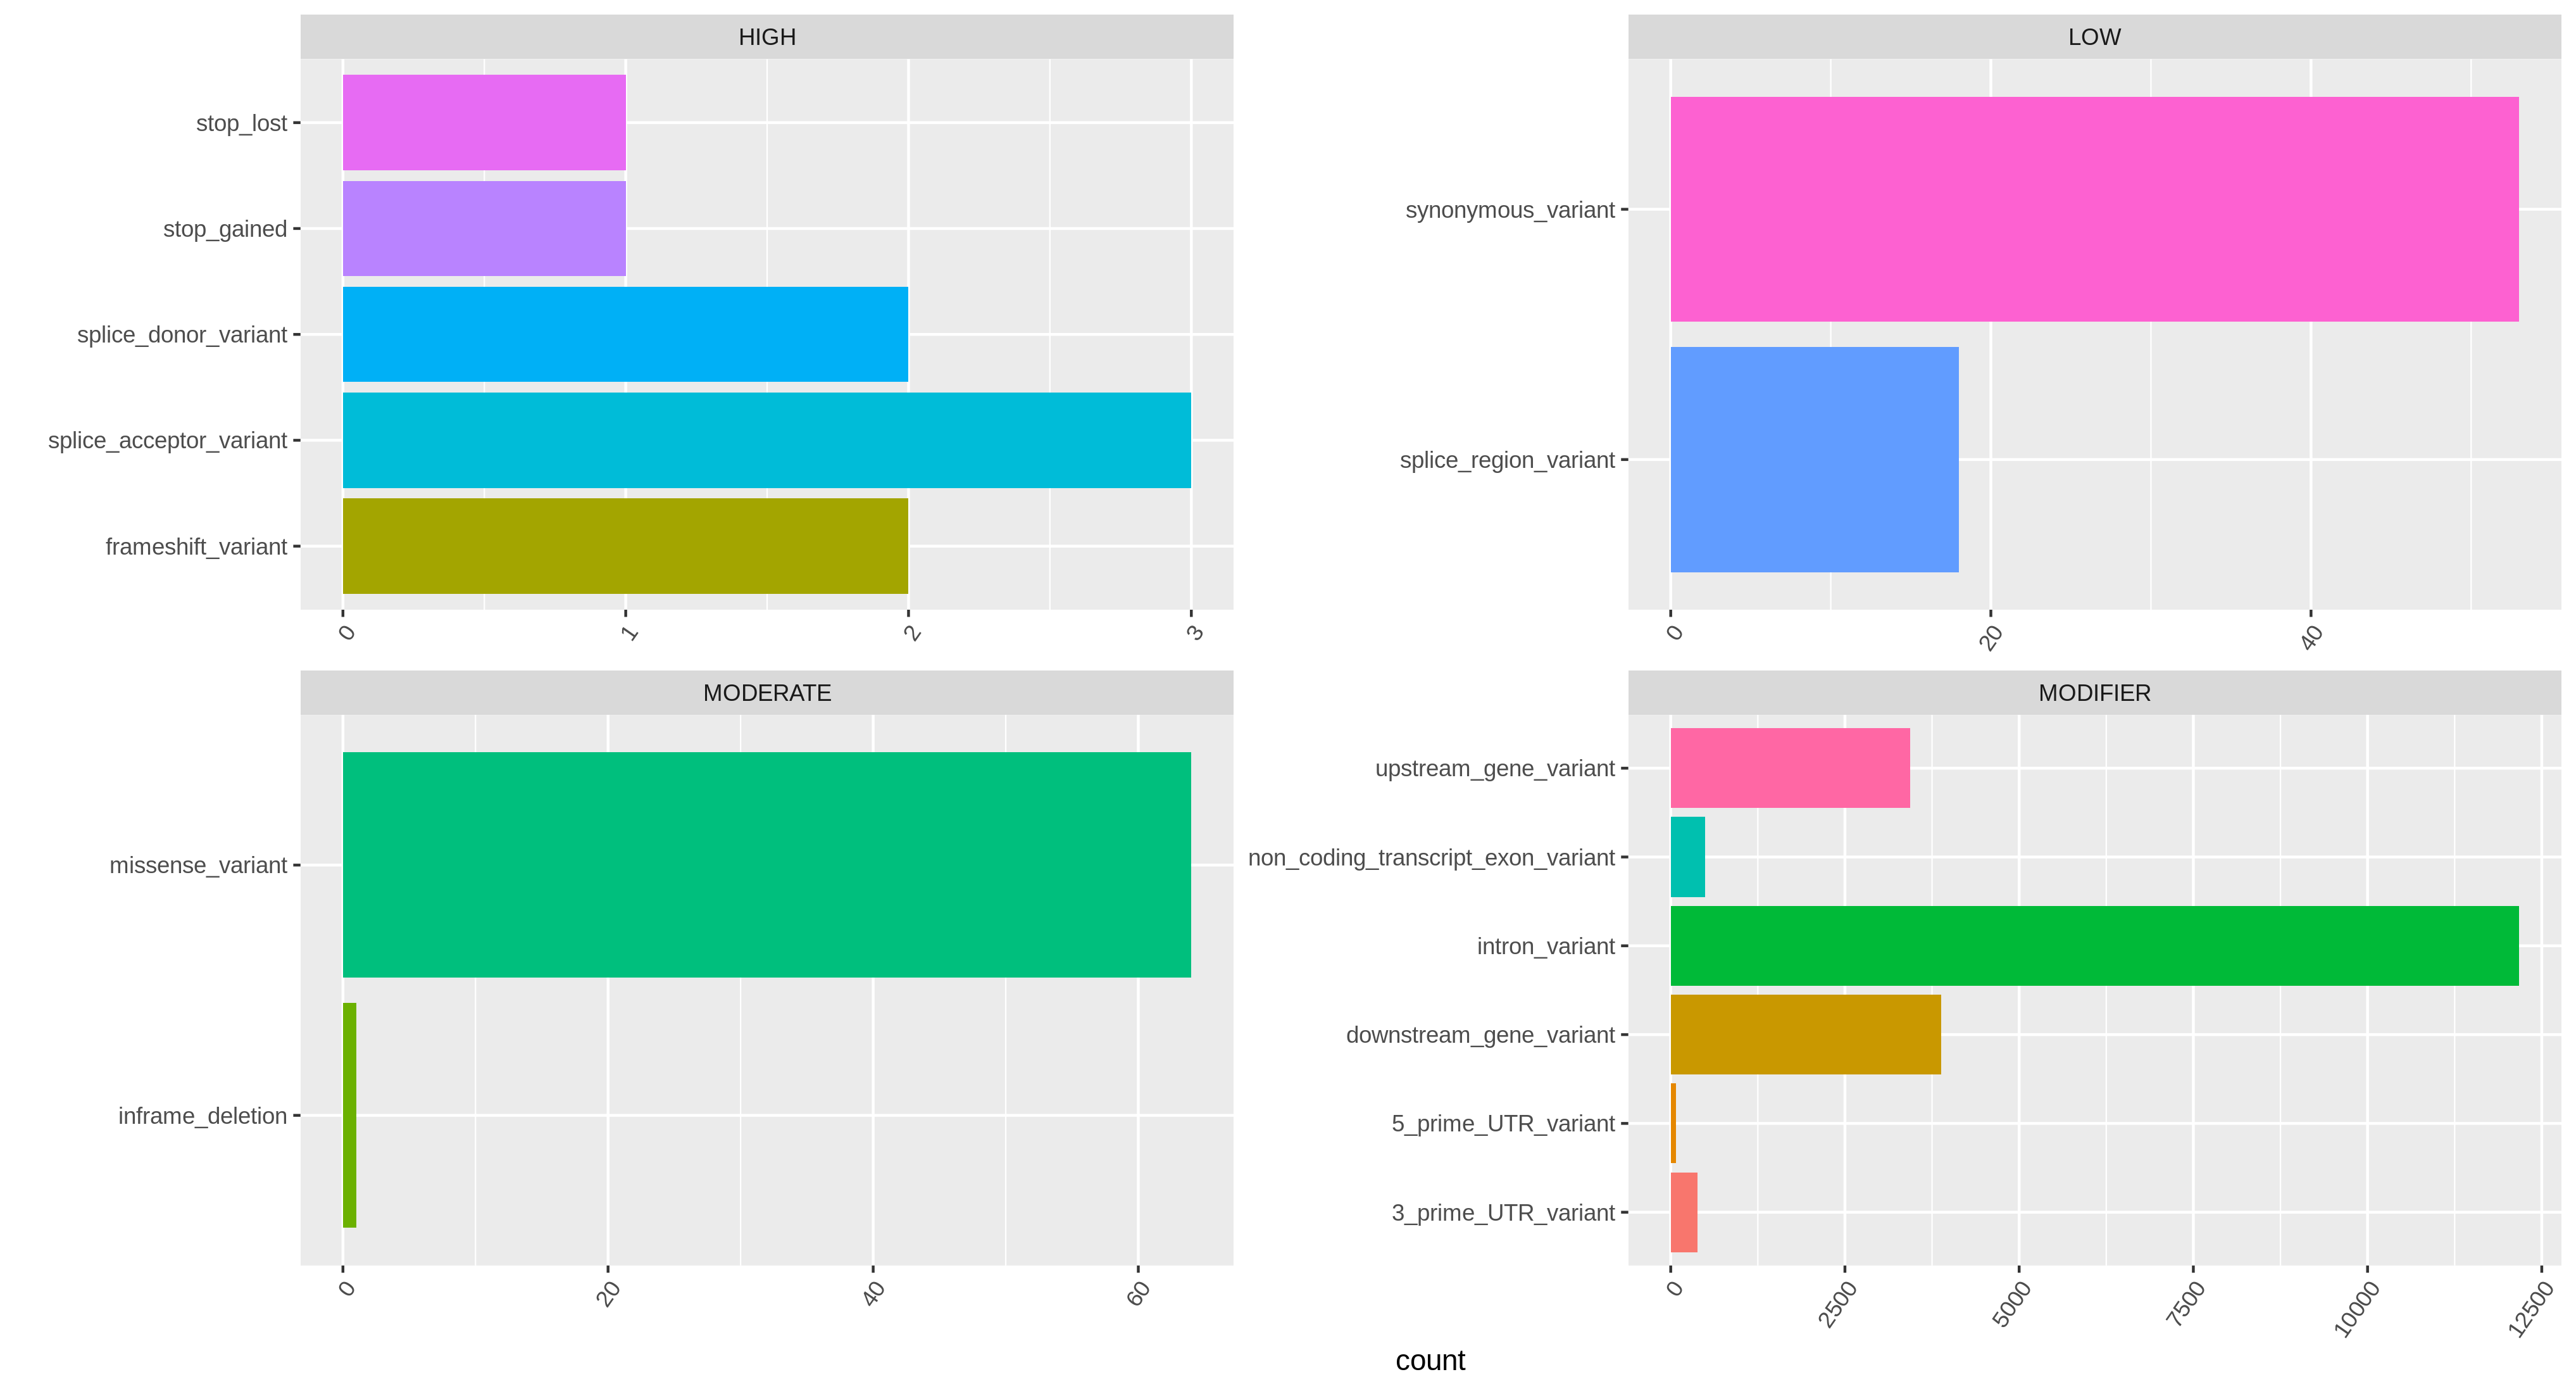
\includegraphics[width=\textwidth]{Fig/consequence.png}
+
\caption{Most severe consequence}
\label{fig:mostsevereconsequence}
\end{figure}\\


{\small
\begin{table}
\caption{High consequence}
\label{tab:MostSevereConsequence}
\centering
\begin{adjustbox}{\textwidth}
\begin{tabular}{c c c c c c c}
\toprule
 \tabhead{Location} & \tabhead{Variation Allele}  & \tabhead{Symbol} & \tabhead{consequence} & \tabhead{Existing variation} \\
\midrule
chr10:133554659 & A/G &  CYP2E1 & non coding transcript variant & rs2149616 \\                                 
chr6:36986144 &  G/- &  MTCH1 & frameshift variant & rs35538959 \\                              
chr3:119503609 & G/C   &  TIMMDC1 & NMD transcript variant & rs1131265 \\                            
chr3:139349435 & G/A  &  MRPS22  & NMD transcript variant & rs10935321\\                          
chr6:131547079 & A/G   &  ARG1  & non coding transcript variant & rs2781646 \\                                
chr17:14102122 & G/A  &  COX10  & NMD transcript variant & rs2159132\\
chr10:50002097 & G/A  & TIMM23B-AGAP6 & non coding transcript variant & rs565737328 \\
chr14:70359741 & T/G &  SYNJ2BP-COX16  & NMD transcript variant & rs17475333 \\
chr14:70049036 & T/- &  SLC8A3 & frameshift variant & NA \\
\bottomrule\\
\end{tabular}
\end{adjustbox}
\end{table}
}



{\small
\begin{table}
\caption{high impact genotypes}
\label{tab.high impact genotypes}
\centering
\begin{tabular}{c c c c c c c c c c c c}
\toprule
\tabhead{Existing variation} & \tabhead{AS006} & \tabhead{AS030} & \tabhead{AS036} & \tabhead{AS054}  & \tabhead{AS064} & \tabhead{AS065} & \tabhead{AS087} & \tabhead{AS090} & \tabhead{AS093} & \tabhead{AS094} & \tabhead{SYMBOL} \\
\midrule 
rs2149616  & 1   &   0    &  0  &    0  &    0   &   1  &    0   &   0   &   2   &   0     & CYP2E1 \\
rs565737328  & 0    &  0     & 0   &   1   &   0    &  0   &   0    &  0   &   0   &   0     & TIMM23B-AGAP6\\
rs17475333  & 0    &  0     & 0  &    0  &    1   &   1   &   0    &  0  &    0   &   0     & SYNJ2BP-COX16\\
rs2159132  & 1    &  0    &  1  &    2  &    1   &   1   &   0    &  2  &    1   &   0    &  COX10\\
rs1131265 & 0    &  1    &  0  &    0  &    0   &   0   &   1   &   0  &    1   &   0    &  TIMMDC1\\
rs10935321 & 0    &  0    &  1  &    0  &    2    &  0   &   1   &   1  &    0   &   2  &   MRPS22\\
rs2781646 & 1   &   0    &  0   &   1   &   0   &   0   &   1   &   0  & 0   &   1  &    ARG1\\

\bottomrule\\
\end{tabular}
\end{table}
}

\subsection{High-impact stop gain mutation in \textit{COX10} and splice donor variant in \textit{MRPS22}}  

Table \ref{tab.high impact genotypes} shows that the high-impact stop gain variant rs2159132 in the Cytochrome c oxidase assembly factor heme A:farnesyltransferase (\textit{COX10}) gene is the most frequent variant among embryos being shared by 7 samples. rs2159132 variant is considered by SIFT as deleterious with a 0 score and by PolyPhen as possibly damaging with a 0.63 score. Cytochrome c oxidase (COX), the terminal component of the mitochondrial respiratory chain, catalyzes the electron transfer from reduced cytochrome c to oxygen. This component is a heteromeric complex consisting of 3 catalytic subunits encoded by mitochondrial genes and multiple structural subunits encoded by nuclear genes. The mitochondrially-encoded subunits function in electron transfer, and the nuclear-encoded subunits may function in the regulation and assembly of the complex.
Deficiencies in the activity of cytochrome c oxidase (COX) are an important cause of autosomal recessive respiratory chain disorders, such as Leigh Syndrome and hypertrophic cardiomyopathy(\cite{antonicka2003mutations}).\\ 


The splice donor variant rs10935321 in the Mitochondrial ribosomal protein S22 (\textit{MRPS22}) it is shared by 5 embryos (Table \ref{tab.high impact genotypes} ).
Mammalian mitochondrial ribosomal proteins are encoded by nuclear genes and help the protein synthesis within the mitochondrion. Mitochondrial ribosomes (mitoribosomes) consist of a small 28S subunit and a large 39S subunit. \textit{MRPS22} encodes a 28S subunit of the mitoribosomes.
\textit{MRPS22} is critical for ovarian development and its study may therefore provide insight into the pathophysiology and treatment of ovarian dysfunction. Pathogenic variants in \textit{MRPS22} can cause primary ovarian insufficiency (POI), defined by the loss or dysfunction of ovarian follicles associated with amenorrhea before the age of 40. POI is a major cause of female infertility with a prevalence greater than 1\% (\cite{chen2018mutations}).\\ 

Following, a brief description of the genes hosting the other high-impact variants I found in my analyses : \\
\textit{CYP2E1}\\
Cytochrome P450 family 2 subfamily E member 1.
This gene encodes a member of the cytochrome P450 superfamily of enzymes. The cytochrome P450 proteins are monooxygenases which catalyze many reactions involved in drug metabolism and synthesis of cholesterol, steroids and other lipids.\\


\textit{MTCH1}\\
Mitochondrial carrier 1
This gene encodes a member of the mitochondrial carrier family. The encoded protein is localized to the mitochondrion inner membrane and induces apoptosis independent of the proapoptotic proteins Bax and Bak.\\

\textit{TIMMDC1}\\
This gene encode for Translocase of inner mitochondrial membrane domain containing 1.
Chaperone protein involved in the assembly of the mitochondrial NADH:ubiquinone oxidoreductase complex (complex I). Participates in constructing the membrane arm of complex I.\\

\textit{ARG1}\\
this gene encode for Arginase 1.
Arginase catalyzes the hydrolysis of arginine to ornithine and urea. At least two isoforms of mammalian arginase exist (types I and II) which differ in their tissue distribution, subcellular localization, immunologic crossreactivity and physiologic function.\\

\textit{TIMM23B}\\
This gene encode for Translocase of inner mitochondrial membrane 23 homolog B and it may participate in the translocation of transit peptide-containing proteins across the mitochondrial inner membrane. the PAM complex (By similarity).\\

\textit{AGAP6}\\
This gene encode for A-kinase anchor protein 6.
The A-kinase anchor proteins (AKAPs) are a group of structurally diverse proteins, which have the common function of binding to the regulatory subunit of protein kinase A (PKA) and confining the holoenzyme to discrete locations within the cell.
The encoded protein is highly expressed in various brain regions and cardiac and skeletal muscle. \\

\textit{SYNJ2BP}\\
This gene encode for Synaptojanin-2-binding protein.
This protein regulates endocytosis of activin type 2 receptor kinases through the Ral/RALBP1-dependent pathway and may be involved in suppression of activin-induced signal transduction. \\


\textit{COX16}\\
This gene encode for COX16, cytochrome c oxidase assembly homolog
Required for the assembly of the mitochondrial respiratory chain complex IV (CIV), also known as cytochrome c oxidase. Promotes the insertion of copper into the active site of cytochrome c oxidase subunit II (MT-CO2/COX2). Interacts specifically with newly synthesized MT-CO2/COX and its copper center-forming metallochaperones SCO1, SCO2 and COA6. Probably facilitates MT-CO2/COX2 association with the MITRAC assembly intermediate containing MT-CO1/COX1, thereby participating in merging the MT-CO1/COX1 and MT-CO2/COX2 assembly lines \\

\textit{SLC8A3}\\
This gene encodes aSolute carrier family 8 member A3
this protein is a member of the sodium/calcium exchanger integral membrane protein family. Na+/Ca2+ exchange proteins are involved in maintaining Ca2+ homeostasis in a wide variety of cell types.\\

\subsection{ Moderate-impact missense variant in \textit{GMF2} }

Almost all variants with moderate impact (65 out of 766,845) are missense variants. For the missense variants, \textsc{vep} annotates also SIFT and PolyPhen scores. The SIFT score ranges from 0.0 (deleterious) to 1.0 (tolerated). The PolyPhen score ranges from 0.0 (tolerated) to 1.0 (deleterious). In my analysis I find 4 deleterious with score zero according to SIFT (Table \ref{tab:SiftDeleterious}), and 9 possibly damaging variants according to PolyPhen (Table \ref{tab:PolyphenDeleterious}).\\


{\small
\begin{table}
\caption{Sift Deleterious missense variants}
\label{tab:SiftDeleterious}
\centering
\begin{tabular}{c c c c c c c}
\toprule
\tabhead{Existing variation} & \tabhead{Position} & \tabhead{Variation} &\tabhead{Gene} \\
\midrule 
rs41304800 & chr20:3147932 & A/C & ENSG00000215251 \\
rs2230351 & chr17:14076741 & A/T  & ENSG00000006695 \\
rs2072279 & chr17:14077033 & G/A & ENSG00000006695 \\ %COX10 
rs2293925 & chr8:143310198 &  G/A  & ENSG00000184428 \\
\bottomrule\\
\end{tabular}
\end{table}
}


{\small
\begin{table}
\caption{Polyphen possibly damaging missense variants}
\label{tab:PolyphenDeleterious}
\centering
\begin{tabular}{c c c c c c c}
\toprule
\tabhead{Existing variation} & \tabhead{Position}  & \tabhead{variation} & \tabhead{Gene} & \tabhead{score}  \\
\midrule 
rs77820367 & chr3:136298060 & G/A & ENSG00000114054  & (0.722) \\
rs77820367 & chr3:136298060 & G/A & ENSG00000114054  & (0.863)\\
rs77820367 & chr3:136298060 & G/A & ENSG00000114054  & (0.793)\\
rs41292543 & chr1:46309111  & A/G & ENSG00000173660   & (0.755)\\
rs41304800 & chr20:3147932 & A/C & ENSG00000215251 & (0.564)\\
rs2072279 & chr17:14077033 & G/A & ENSG00000006695  & (0.63)\\ %COX10
rs16872235 & chr5:74741561 & T/A & ENSG00000164347  & (0.907)\\
rs16872235 & chr5:74741561 & T/A & ENSG00000164347 & (0.849)\\
rs2293925  & chr8:143310198 & G/A & ENSG00000184428 & (0.586)\\
\bottomrule\\
\end{tabular}
\end{table}
}

The variant rs16872235 in the mitochondrial Ribosome-releasing factor 2 (\textit{GFM2}) it is the most deleterious according to PolyPhen with 0.907 score  (Table \ref{tab:PolyphenDeleterious}) and it is considered by SIFT as deleterious with 0.02 score.
\textit{GFM2} encodes one of the mitochondrial translation elongation factors, which is a GTPase that plays a role at the termination of mitochondrial translation by mediating the disassembly of ribosomes from messenger RNA. 
Defects in the mitochondrial translation machinery caused by
genetic mutations have been implicated in respiratory deficiency,
which is an underlying factor in a number of diseases including Leigh syndrome. 
Mitochondrial disease caused by \textit{GFM2} mutations could be characterized by arthrogryposis multiplex congenita and bradycardia, because the \textit{GFM2} protein is highly expressed in skeletal muscle,the heart and fetal liver, which contain a large number of mitochondria. (\cite{fukumura2015compound}) \\




\begin{figure}[h]
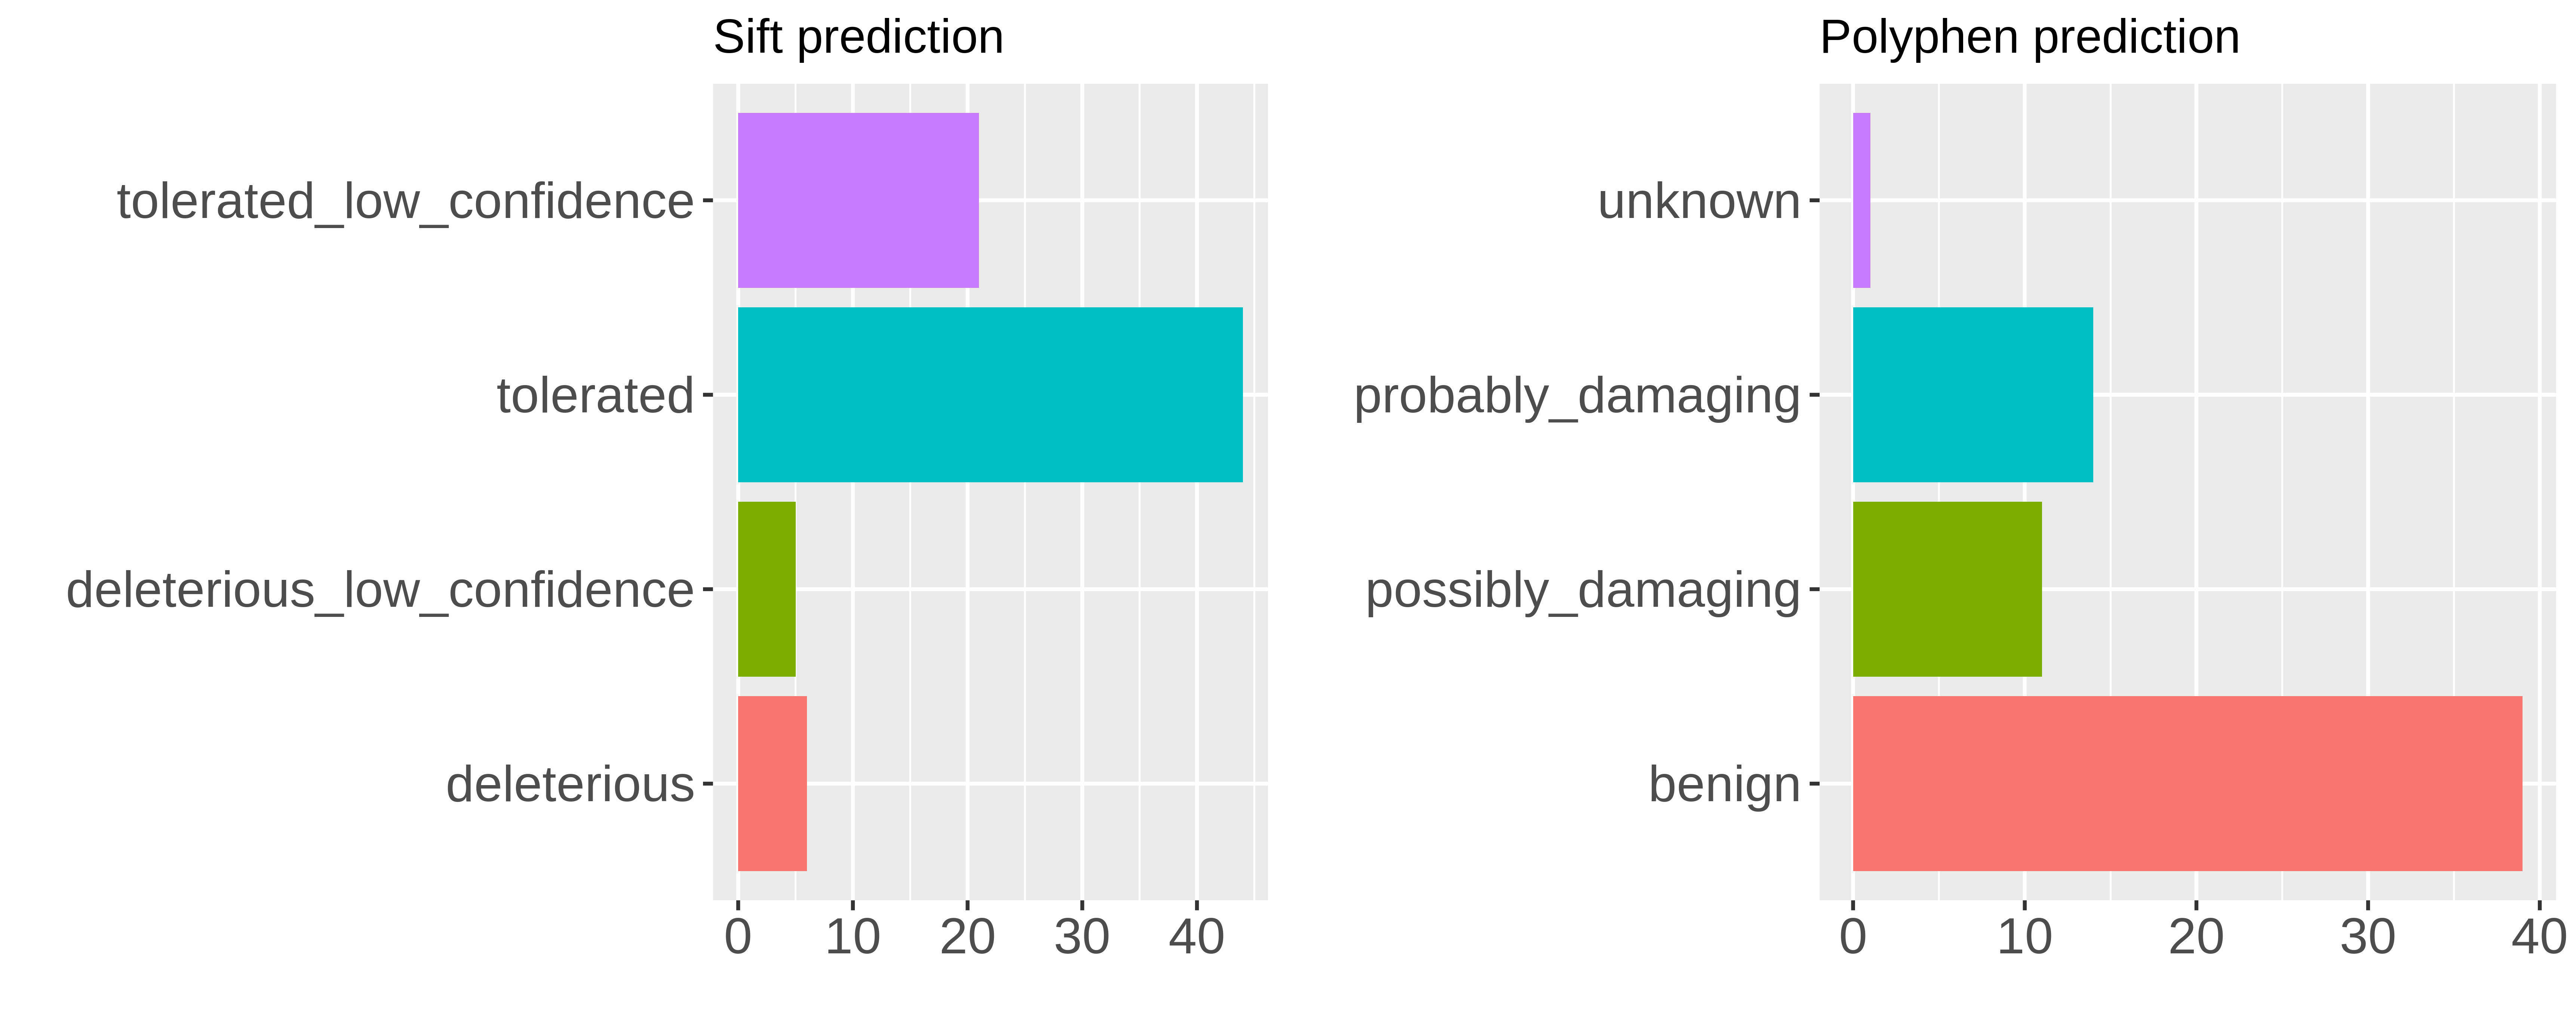
\includegraphics[width=\textwidth]{Fig/nuclear_SiftPoly.png}
\caption{Sift and Polyphen Nuclear Gene}
\label{fig:siftpolyphen_nuclear}
\end{figure}\\





\section{Haplogroup}
The mtDNA can be classified into phylogenetic clusters, called Haplogroups.
Haplogroup is a group of similar haplotypes that share common ancestor, i.e. share some Single Nucleotide Polymorphism (SNP) mutations. It's called haplotype because it is only present in one chromosome of the pair, that is, in a haploid state. If a sufficient number of individuals are examined for their haplotypes, maps can be created, showing the distribution of various haplogroups across the world. These maps are called Haplotype Maps (Figure \ref{fig:Haplogroups}), contain information about the order in which SNPs appeared through time, and they provide a variety of information, such as the ethnic makeup of a population, the history of past migrations of people to different parts of the world, etc. (\cite{arora2015hgsdb})\\
The regionality of the mtDNA haplogroups is important in several aspects. First, of all of the African diversity, only two mtDNA lineages (M and N) colonized the rest of the world. Second, of all of the Asian mtDNAs, only three mtDNA lineages (A, C, and D) moved to extreme northeast Siberia to found the Paleo-Indians. Third, the mtDNA sequence evolution rate is such that it produced important mtDNA evolutionary changes that coincide with the major human geographic migrations. Such associations could not have occurred by chance. Rather, it is most likely that mtDNA variation permitted adaptation of our human ancestors to different regional environments, thus being the adaptive system that permitted human colonization of the diverse environments that they encountered around the globe. (\cite{wallace2013mitochondrial})\\



{\small
\begin{table}
\caption{Haplogroups Location Tab}
\label{tab:Haplogroups}
\centering
\begin{tabular}{c c c c c c c}
\toprule
\tabhead{Geographic Location} & \tabhead{Haplogroup}\\
\midrule 
African &  L0, L1, L2, L3, L4, L5, L6   \\
West Eurasian & H, T, U, V, X, K, I, J, W.   \\
East Eurasian & A, B, C, D, E, F, G, Y, Z.\\
Native American & A, B, C, D, X \\
\bottomrule\\
\end{tabular}
\end{table}
}



\begin{figure}[H]
\centering
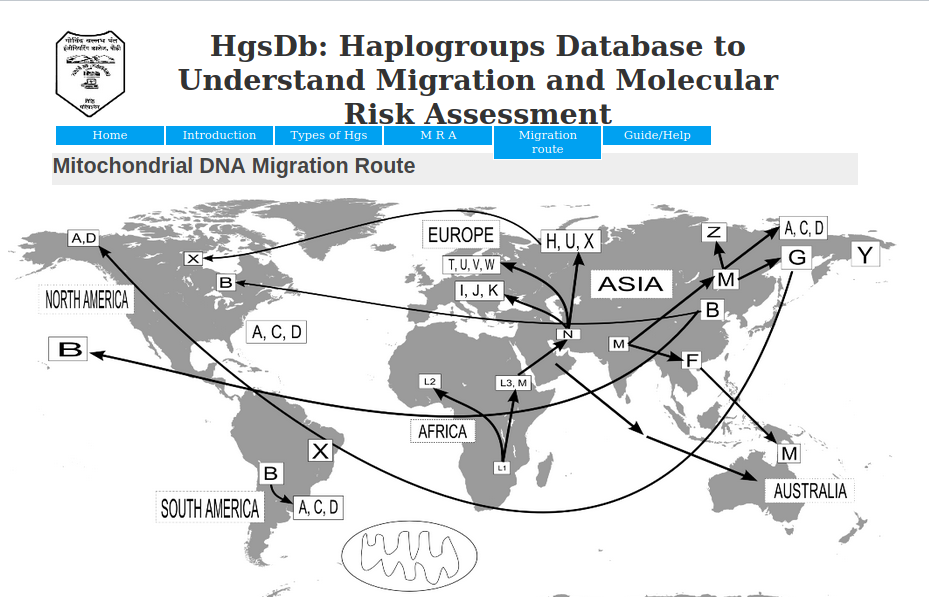
\includegraphics[width=1\textwidth]{Fig/HaplogroupsMigration.png}
\decoRule
\caption{\textbf{}} \textit{ Adapted from \cite{arora2015hgsdb}}. 
\label{fig:Haplogroups}
\end{figure} 

%\begin{figure}[H]
%\centering
%\includegraphics[width=\textwidth]{Fig/MtDNA_haplogroup_tree_and_di%stribution_map.png}
%\decoRule
%\caption{\textbf{}} \textit{ Adapted from %\cite{kivisild2015maternal}}. 
%\label{fig:Haplogroups}
%\end{figure} 



To define the haplogroups in my data I used \textsc{Haplogrep}, a haplogroup classification tool (\cite{weissensteiner2016haplogrep}). The majority of sequences (n=6) belong to haplogroup H, typical of West Eurasia. One sequence belong to haplogroup L, typical of Africa, and two to haplogroups M and N which are commonly found in Asia. My findings are concordant with the demographic data that were avaialble for these samples.  




{\small
\begin{table}
\caption{Haplogroups}
\label{tab:Haplogroups}
\centering
\begin{tabular}{c c c c c c c}
\toprule
\tabhead{Sample ID} & \tabhead{Haplogroup} & \tabhead{Subgroup}\\
\midrule 
AS006 & H &  H2a2a   \\
AS030 & H &  H       \\
AS036 & H &  H7b1   \\
AS054 & L &  L1c3    \\
AS064 & H &  H+152    \\
AS065 & N &   N1a1    \\
AS074 & H &   H+152   \\
AS087 & M & M5a2a1a1   \\
AS090 & T &  T2b3+151  \\
AS093 & T &   T2c1   \\
AS094 & H &    H     \\
\bottomrule\\
\end{tabular}
\end{table}
}


\subsection{Heteroplasmy}


Mitochondrial heteroplasmy is defined as a dynamically determined co‐expression of wild-type (WT)‐inherited polymorphisms and somatic mutations in varying ratios within individual mtDNA genomes distributed throughout the intraorganelle compartments of individual cells. (\cite{stefano2016mitochondrial})
Many pathogenic mtDNA mutations have been identified and the most severe mutations are heteroplasmic.
Heteroplasmic alleles can shift in percentage during both mitotic and meiotic cell division, leading to a potentially continuous
array of bioenergetic defects, this process is known as replicative segregation. As the percentage of mutant mtDNAs increases, the resulting bioenergetic defect becomes increasingly severe. An example of the interaction between mtDNA heteroplasmy variation and phenotype was the report that the tRNA Lys nt 8344A.G  mutation that causes myoclonic epilepsy and ragged red fiber (MERRF) disease was heteroplasmic (\cite{wallace2013mitochondrial}) \\
The effect of mtDNA mutant heteroplasmy on phenotype is even more striking with the tRNA Leu(UUR) mt 3243A.G mutation associated with mitochondrial encephalomyopathy, lactic acidosis, and stroke-like episodes (MELAS) (\cite{goto2011dynamics}). When the heteroplasmy of this mutation is high, it can present as lethal childhood Leigh syndrome, MELAS, chronic progressive external ophthalmoplegia (CPEO),cardiomyopathy, migraines, diabetes mellitus,and deafness. In pedigrees with high heteroplasmy members, meiotic segregation of the mutant mtDNAs can result in the full range of phenotypes from asymptomatic to lethal disease.
(\cite{wallace2013mitochondrial})\\

To evaluate heteroplasmy in my data, I used \textsc{Mity - report} (\cite{puttick2019mity}). 
The file I obtained contains several parameters for determining heteroplasmy. One of the parameters is the genotype. I have chosen to consider those with the 0/1 genotype as heteroplasmic variants. Overall, the report identified 231 heteroplasmic sites. Among these, the percentage of heteroplasmy varies from a minimum of 0.000100  to a maximum of 0.999900.
As explained in figure \ref{fig:distributionHet} 

\begin{figure}[H]
\centering
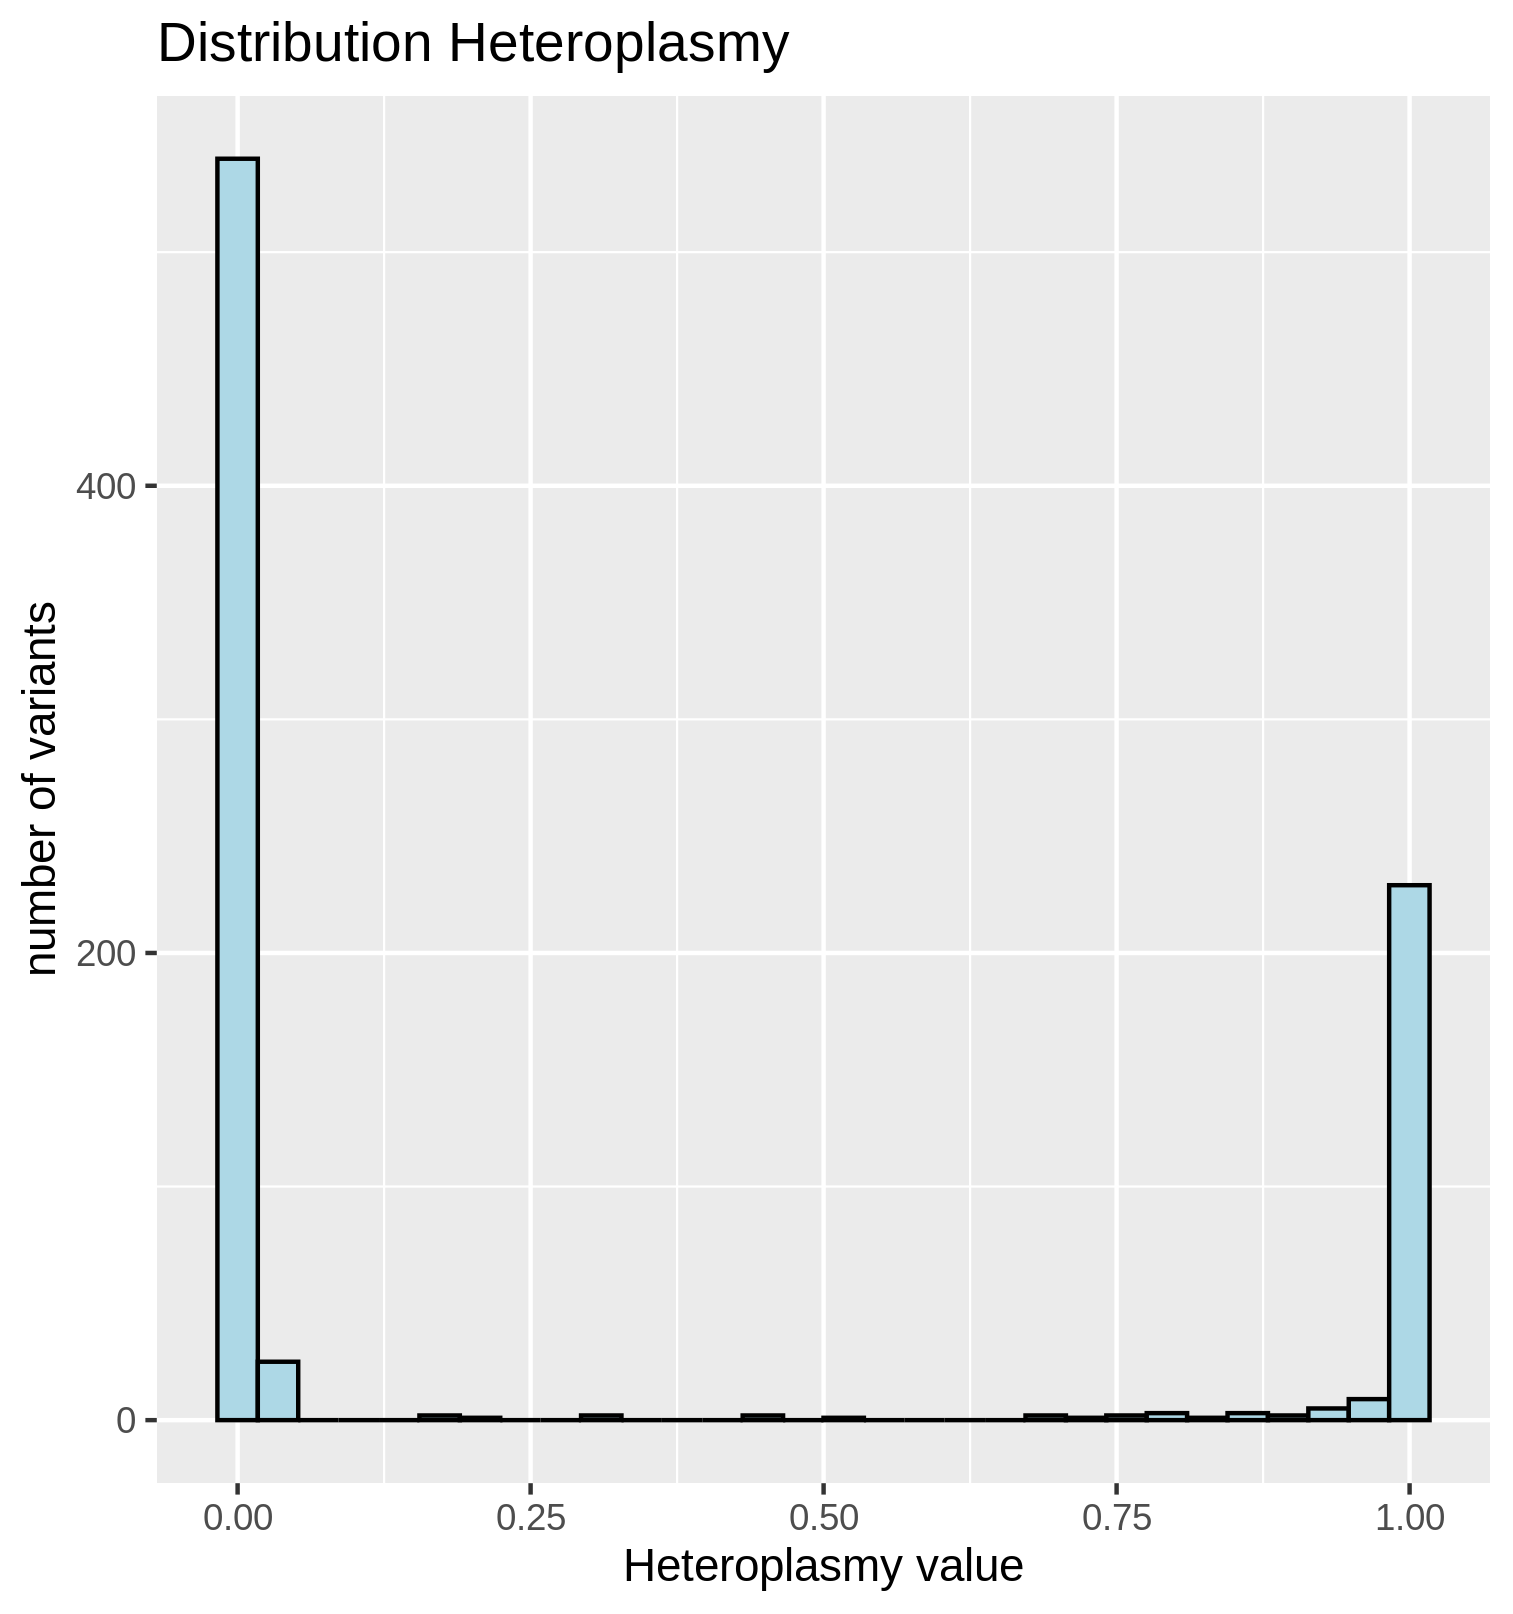
\includegraphics[width=\textwidth]{Fig/histogram.png}
\decoRule
\caption{\textbf{}} \textit{\cite{}}. 
\label{fig:distributionHet}
\end{figure} 

(modificando la soglia, impostandola ad es > 0.05 e < 0.80 trovo 15 varianti) \\ 


\begin{figure}[H]
\centering
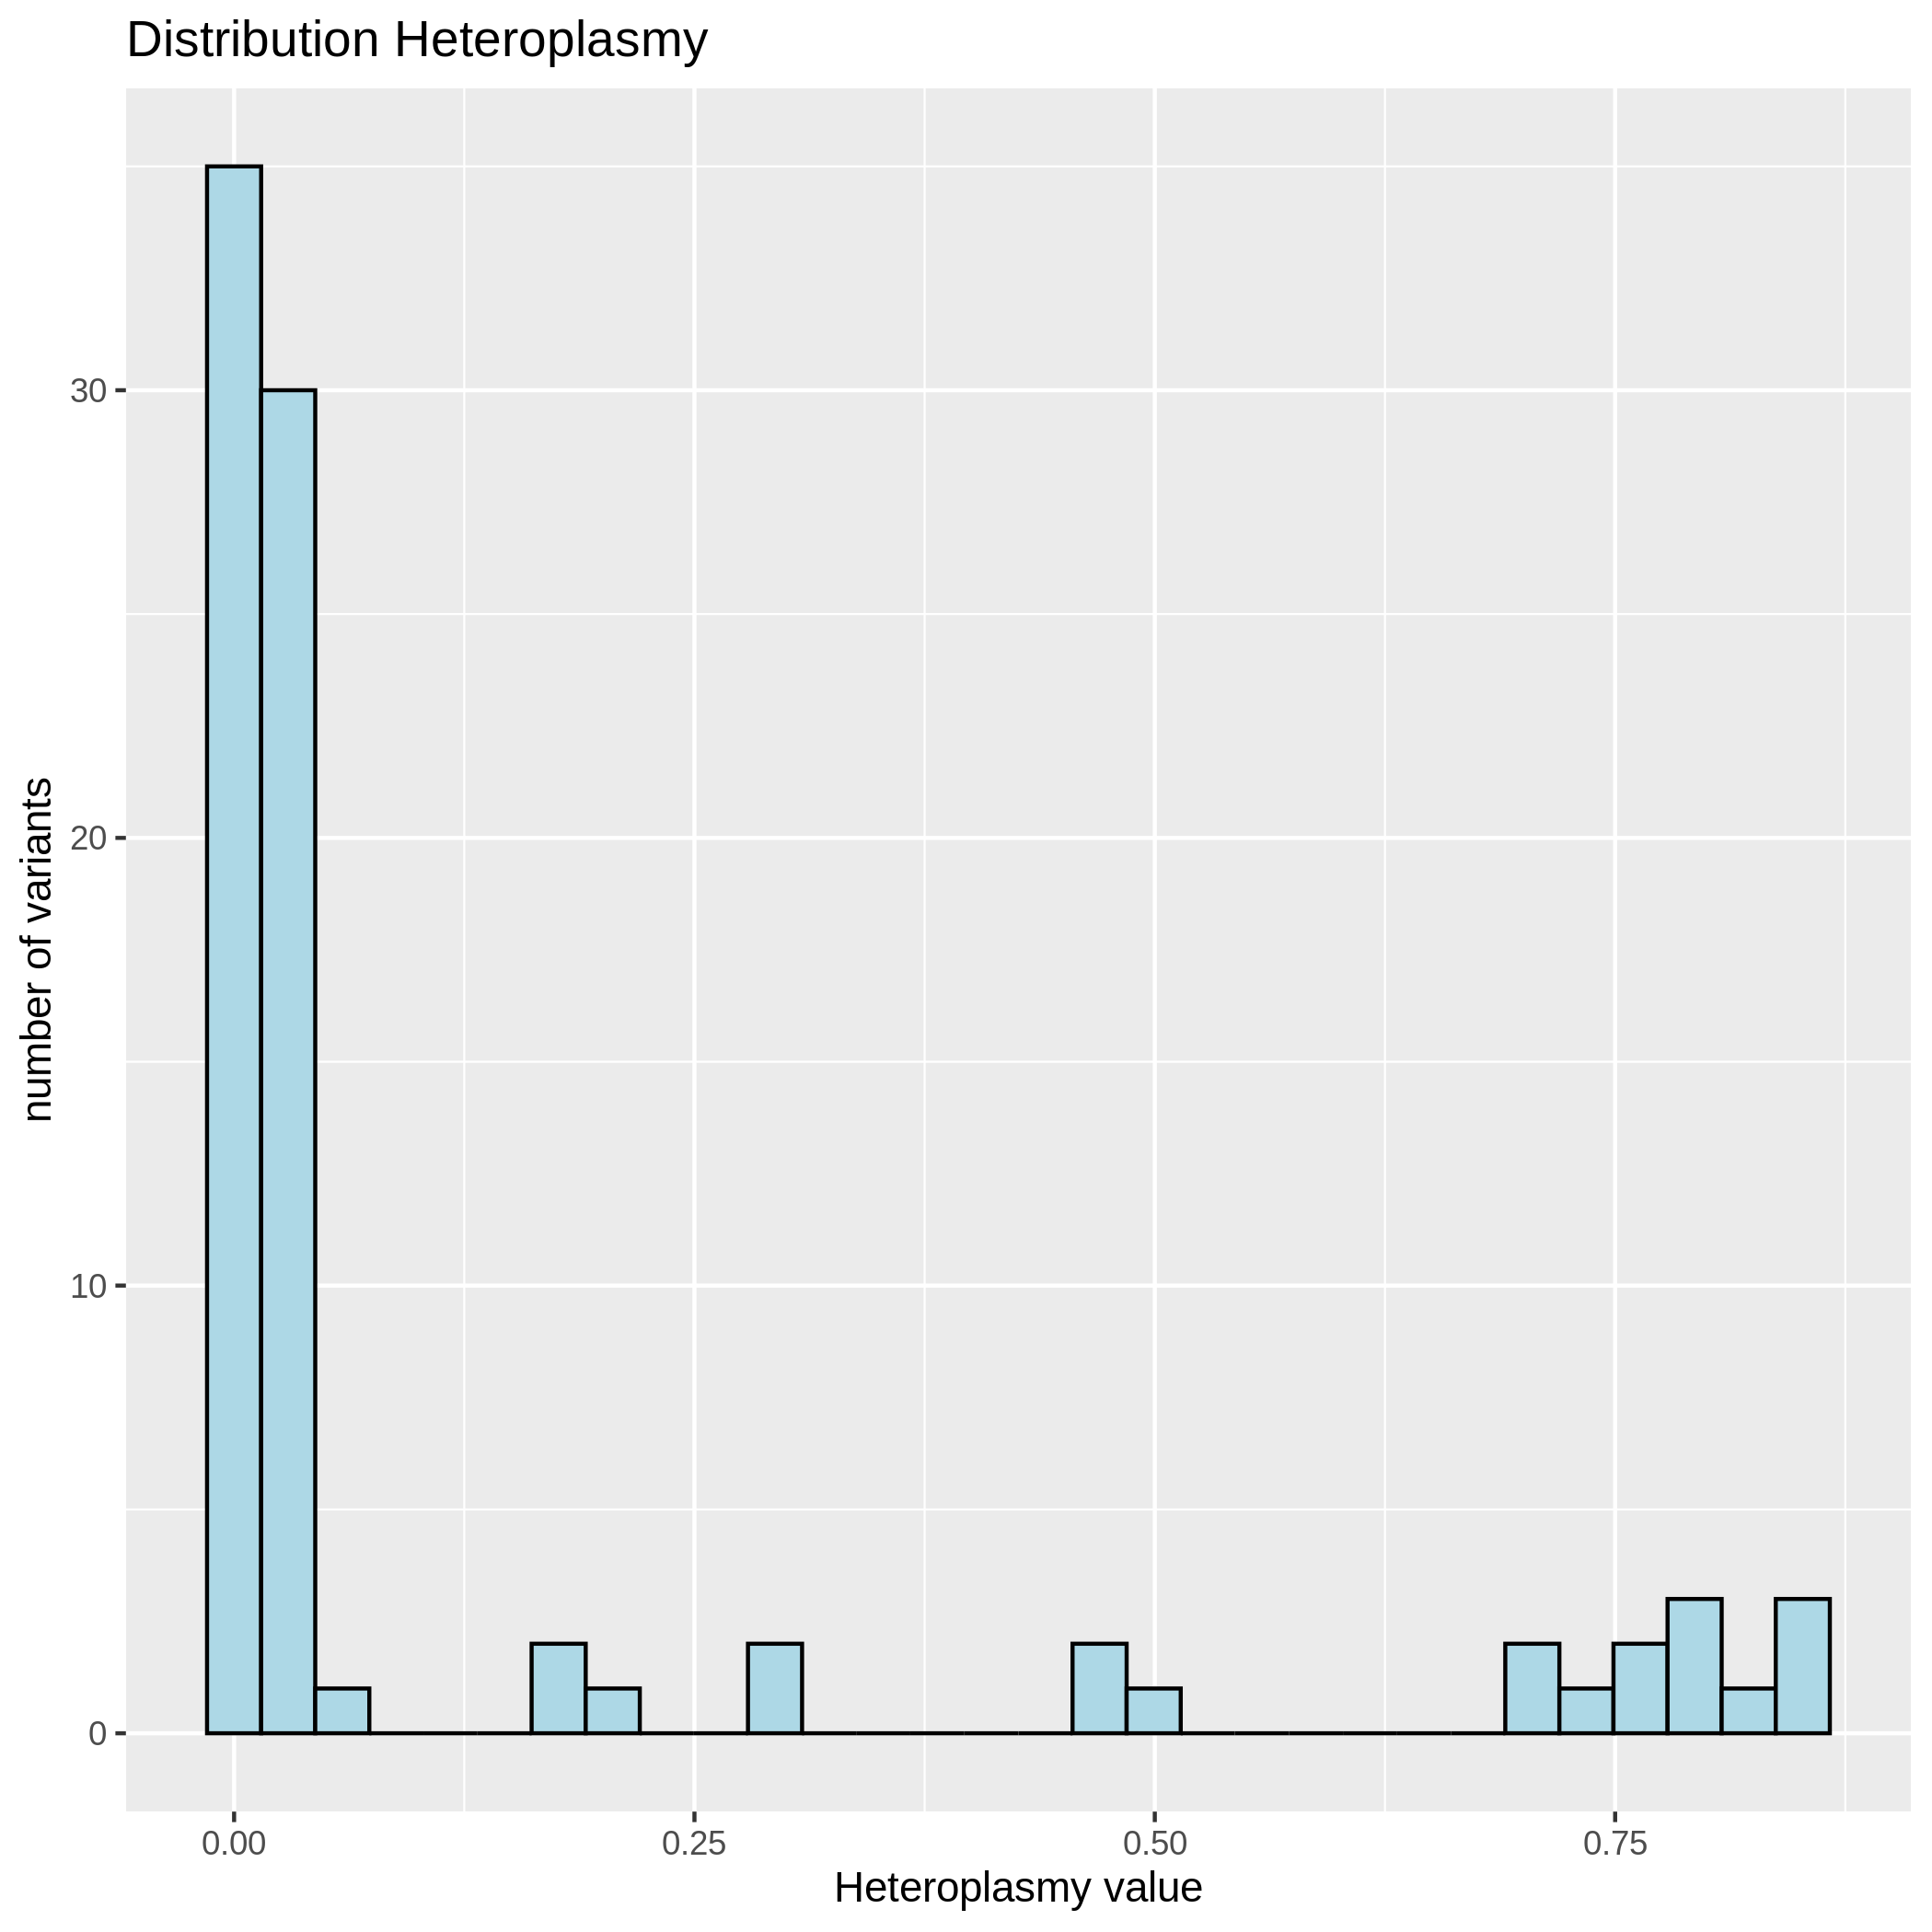
\includegraphics[width=\textwidth]{Fig/dist_heteroplasmy_from-01-90.png}
\decoRule
\caption{\textbf{}} \textit{\cite{}}. 
\label{fig:distributionHet}
\end{figure} 


I have considered heteroplasmy in the four missense variants \ref{tab:missense} to determine any pathogenity linked to. \\

{\small
\begin{table}
\caption{Heteroplasmy}
\label{tab:Haplogroups}
\centering
\begin{tabular}{c c c c c c c}
\toprule
\tabhead{Variant} & \tabhead{Number of samples} & \tabhead{Min Heteroplamsy} & \tabhead{Max Heteroplasmy}\\
\midrule 
5374  & 5   & 0.0003    &  0.0156  \\
8668  & 2   & 0.0001    &  0.9998    \\
14447 & 6   & 0.0003    &  0.0287   \\
14556 & 8   & 0.0003    &  0.0117   \\
\bottomrule
\end{tabular}
\end{table}
}






\include{Chapters/discussion}

\chapter{Methods}

\section{Data and sample collection.} 
Study material consisted in blood and and product of conception from the mothers and was collected at the Section Unit of Obstetrics and Gynecology at the University Hospital of Ferrara. The study was approved by the ethical committee of the Emilia-Romagna and was carried out in compliance with the Helsinki Declaration. All participants provided written informed consents prior to recruitment. All patient data were anonymized right after data and sample collection.\\ 

%Data were cleaned and refined (e.g.trimming of white spaces, correction of typing errors, harmonization of values within fields, and similar) using OpenRefine (\url{https://github.com/OpenRefine/OpenRefine}), a standalone open source application for data cleanup and transformation (\href{https://en.wikipedia.org/wiki/OpenRefine}{wiki}).\\

Summary statistics of the data were calculated and represented using the R packages \textit{ggplot} (\cite{ggplot2}), \textit{tidyverse} (\cite{wickham2019welcome}), \textit{stats} (\cite{statsR}) and \textsc{r} (\cite{R}). All the code is availabe on the git repository of the project (\url{https://github.com/ezcn/grep}) 

\section{Screening for chromosomal aneuploidies}
This part was performed by our collaborators at the University of Ferrara and Merigen Reserach s.r.l. In brief DNA was extracted from chorionic villi of the product of conception using standard protocols. A rapid screening of sex and numerical anomalies for chromosomes 13, 15, 16, 18, 21, 22 and X was carried out with the miscarriage DNA samples performing quantitative PCR assays. Samples that resulted euploid for these chromosomes were further analized by Comparative Genomic Hybridization (Agilent SurePrint G3) and low coverage sequencing of randomly amplified genomic regions


\section {Whole-genome sequencing and sequence analyses}

%\subsection{Sequencing}
Sequencing was done through a service provider (Macrogen s.r.l). In particular, libraries for sequencing were prepared using the Illumina TruSeq DNA PCR-free Library (insert size 350bp) and samples were sequenced at 30X mapped (~110Gb) 150bp PE on HiSeqX. Data were released in as fastq files. 

\textbf{Alignment with reference.} Reads in the fastq file were aligned against the reference genome GRChg38.p12 (\cite{rosenbloom2015ucsc}) using \textsc{bwa} and \textsc{samtools}. \textsc{bwa} (\url{https://github.com/lh3/bwa}) is a software package for mapping low-divergent sequences against a large reference genome, such as the human genome. Of the three algorithms available in \textsc{bwa} we used \textsc{bwa-mem}  that is generally recommended to analyze 70-100bp Illumina reads. 

For each sample, the following command line takes in input fastq file (paired-end) and gives as output a raw-bam file. 

\begin{verbatim}
~/bin/bwa mem -t 16 -R "@RG\tID:$idsample\tSM:$idsample" \
hg38.p12.fa \ 
$namedir/$nameflgz1 \ 
$namedir/$nameflgz2 | \ 
samtools view -b - > \
samples/%$idsample.raw.bam
\end{verbatim}
  


\textsc{samtools} (\url{https://github.com/samtools/samtools}) is a set of utilities for interacting with and post-processing short DNA sequence read alignments in the SAM (Sequence Alignment/Map), BAM (Binary Alignment/Map) and CRAM formats (\href{https://en.wikipedia.org/wiki/SAMtools}{wiki}). \newline
We have used this software downstream \textsc{bwa-mem} for obtain the BAM from fastq. \newline

\textbf{Remove PCR duplicate.} During PCR the machine introduces a several PCR duplicate in our sequence, for remove them we have used SAMbamba (\url{https://github.com/biod/sambamba}) a high performance highly parallel robust and fast tool (and library), written in the D programming language, for working with SAM and BAM files. Current functionality is an important subset of samtools functionality, including view, index, sort, markdup, and depth (\href{https://github.com/biod/sambamba#introduction}{git}). We have used the function markdup to remove PCR duplicates. \newline

%\begin{verbatim}
%~/bin/sambamba markdup -t 8 -p  \
%--tmpdir /scratch --overflow-list-size 500000 \
%/mpbastudies3/IMMA/samples/${idflrbam}.raw.sorted.bam \
%/mpbastudies3/IMMA/samples/${idflrbam}.bam    
%\end{verbatim}

%The command line takes in input a raw version of the BAM file for each sample and gives us as output the BAM file without PCR duplicates. \newline

\textbf{VariantCalling.} Is the process that allows us to identifies sites that differ from the reference for each sample. I have choose \textsc{MITY} (\cite{puttick2019mity}) a pipeline for detecting and interpreting heteroplasmic SNVs and INDELs in the mitochondrial genome using WGS data.Mity is a bioinformatic analysis pipeline designed to call mitochondrial SNV and INDEL variants from Whole Genome Sequencing (WGS) data and it can also identify very low-heteroplasmy variants, even <1\% heteroplasmy when there is sufficient read-depth (eg >1000x). Mity  takes as input bam files and give as output a table with value for each site. The option I used is -mitycall. \textsc{MITY} is based on the \textsc{freebayes} algorithm (\url{https://github.com/ekg/freebayes}) that is a Bayesian genetic variant detector designed to find small polymorphisms, specifically SNPs (single-nucleotide polymorphisms), indels (insertions and deletions), MNPs (multi-nucleotide polymorphisms), and complex events (composite insertion and substitution events) smaller than the length of a short-read sequencing alignment (\href{https://github.com/ekg/freebayes}{git}).
To find heteroplasmy in our saple, I used Mity.
Mity can identify very low-heteroplasmy variants, even <1\% heteroplasmy when there is sufficient read-depth (eg >1000x). \newline

\begin{verbatim}
~/lustrehome/giuliana/anaconda3/bin/mity call --reference hg38 \
--normalise /lustre/home/enza/grep/bam/$1.bam --out-folder-path \
/lustrehome/giuliana/mity/mitycall/ && touch \
/lustrehome/giuliana/error/$1.mitycall_ok \
\end{verbatim}

To use this command line is necessary the reference genome (hg38.p12) in fasta format and a BAM for each sample. 

\begin{verbatim}
~/lustrehome/giuliana/anaconda3/bin/mity report \
/lustrehome/giuliana/mity/mitycall/$1.mity.vcf.gz --out-folder-path
/lustrehome/giuliana/mity/mitycall/mityreport/ && touch \
/lustrehome/giuliana/error/$1.mitycall_ok \
\end{verbatim}

\textbf{Compress and indexing.} When a file was generated is necessary do a compressing and indexing for each one. \newline

Bgzip (\url{https://www.htslib.org/doc/bgzip.html#DESCRIPTION}) compresses files into a series of small (less than 64K) 'BGZF' blocks. This allows indexes to be built against the compressed file and used to retrieve portions of the data without having to decompress the entire file (\href{https://www.htslib.org/doc/bgzip.html#DESCRIPTION}{wiki}). \newline 

%\begin{verbatim}
%~/bin/bgzip /mpbastudies3/IMMA/samples/vcf/${idsample}.vcf > \
%/mpbastudies3/IMMA/samples/vcf/${idsample}.vcf.gz
%\end{verbatim}

The command line take in input the output (VCF) from variant calling and give us the compressed file. \newline 

Tabix (\url{https://www.htslib.org/doc/tabix.html}) indexes a
TAB-delimited genome position file in.tab.bgz and creates an index file.\newline

\begin{verbatim}
%~/bin/tabix -p vcf
/mpbastudies3/IMMA/samples/vcf/${id}.${chr}.vcf.gz 
%\end{verbatim}

The command line take in input the compressed file from BGZIP and give the indexed one.\newline

\textbf{Variant Effect Predictor.}  VEP (\url{https://grch37.ensembl.org/info/docs/tools/vep/index.html}) determines the effect of your variants (SNPs, insertions, deletions, CNVs or structural variants) on genes, transcripts, and protein sequence, as well as regulatory regions.
Simply input the coordinates of your variants and the nucleotide changes to find out the:
\begin{itemize}
    \item Alleles, Genes and Transcripts affected by the variants
    \item Location of the variants (e.g. upstream of a transcript, in coding sequence, in non-coding RNA, in regulatory regions)
    \item Consequence of your variants on the protein sequence (e.g. stop gained, missense, stop lost, frameshift)
    \item Known variants that match yours, and associated minor allele frequencies from the 1000 Genomes Project
    \item  SIFT and PolyPhen-2 scores for changes to protein sequence
\end{itemize}
\newline
This software takes in input a final version of the VCF (filtered) and gives to us an annotated version with all the parameters written in the command-line. \newline

\begin{verbatim} ~ /bin/singularity exec -B /lustre/home/enza -B   /lustrehome/giuliana
/lustre/home/enza/biocontainers/vep100_CADD.img vep --af_1kg  /
--af_gnomad --appris --biotype --buffer_size 5000 --check_existing
/ --distance 5000 --fork 4 --minimal --polyphen b --pubmed
--regulatory --sift b --species homo_sapiens --symbol --tsl --cache
/ --dir_cache /lustre/home/enza/biocontainers/vepcache --offline /
--tab  --variant_class -i
/lustrehome/giuliana/mity/mitycall/mergedfrombam/ALL2.mity.vcf -o /lustrehome/giulian
a/mity/mitycall/mergedfrombam/ALL2.mit
y.vep.tab 

\end{verbatim}\\


\subsection{Haplogroup determination}
HaploGrep 2 supports the direct import of VCF files, one of the current standard formats for genetic data.
Haplogrep requires Java 8 and works on Windows, Linux and Mac. and gives to us a text file with all the parameters written in the command line. \newline

\begin{verbatim} 
java -jar haplogrep-2.1.25.jar --in \
/home/obilab/giuliana/samples_mt/ALLsamples.mity.filt.vcf.gz \
--format vcf --out ALLsamples_haplogroups.txt \ \end{verbatim}
\\
\textbf{}



\newline

 \ref{fig:bmi} .\newline

 \ref{fig:pipeline_screening}).\newline

 \ref{fig:aneuploidies_CHG}).\newline




\printglossary
\begin{acknowledgements}
\addchaptertocentry{\acknowledgementname}
\end{acknowledgements}







\end{document}


